\chapter{Data Analysis}

\section{Target Position Correction}

\indent The information obtained from the MWPCs has been used to accurately determine the positions of the targets. The reaction vertex has been obtained from the analysis of charged tracks which come from the reaction of the photon with the target. The results of this reconstruction are presented in the below figures:

\begin{figure}[H]
\begin{center}
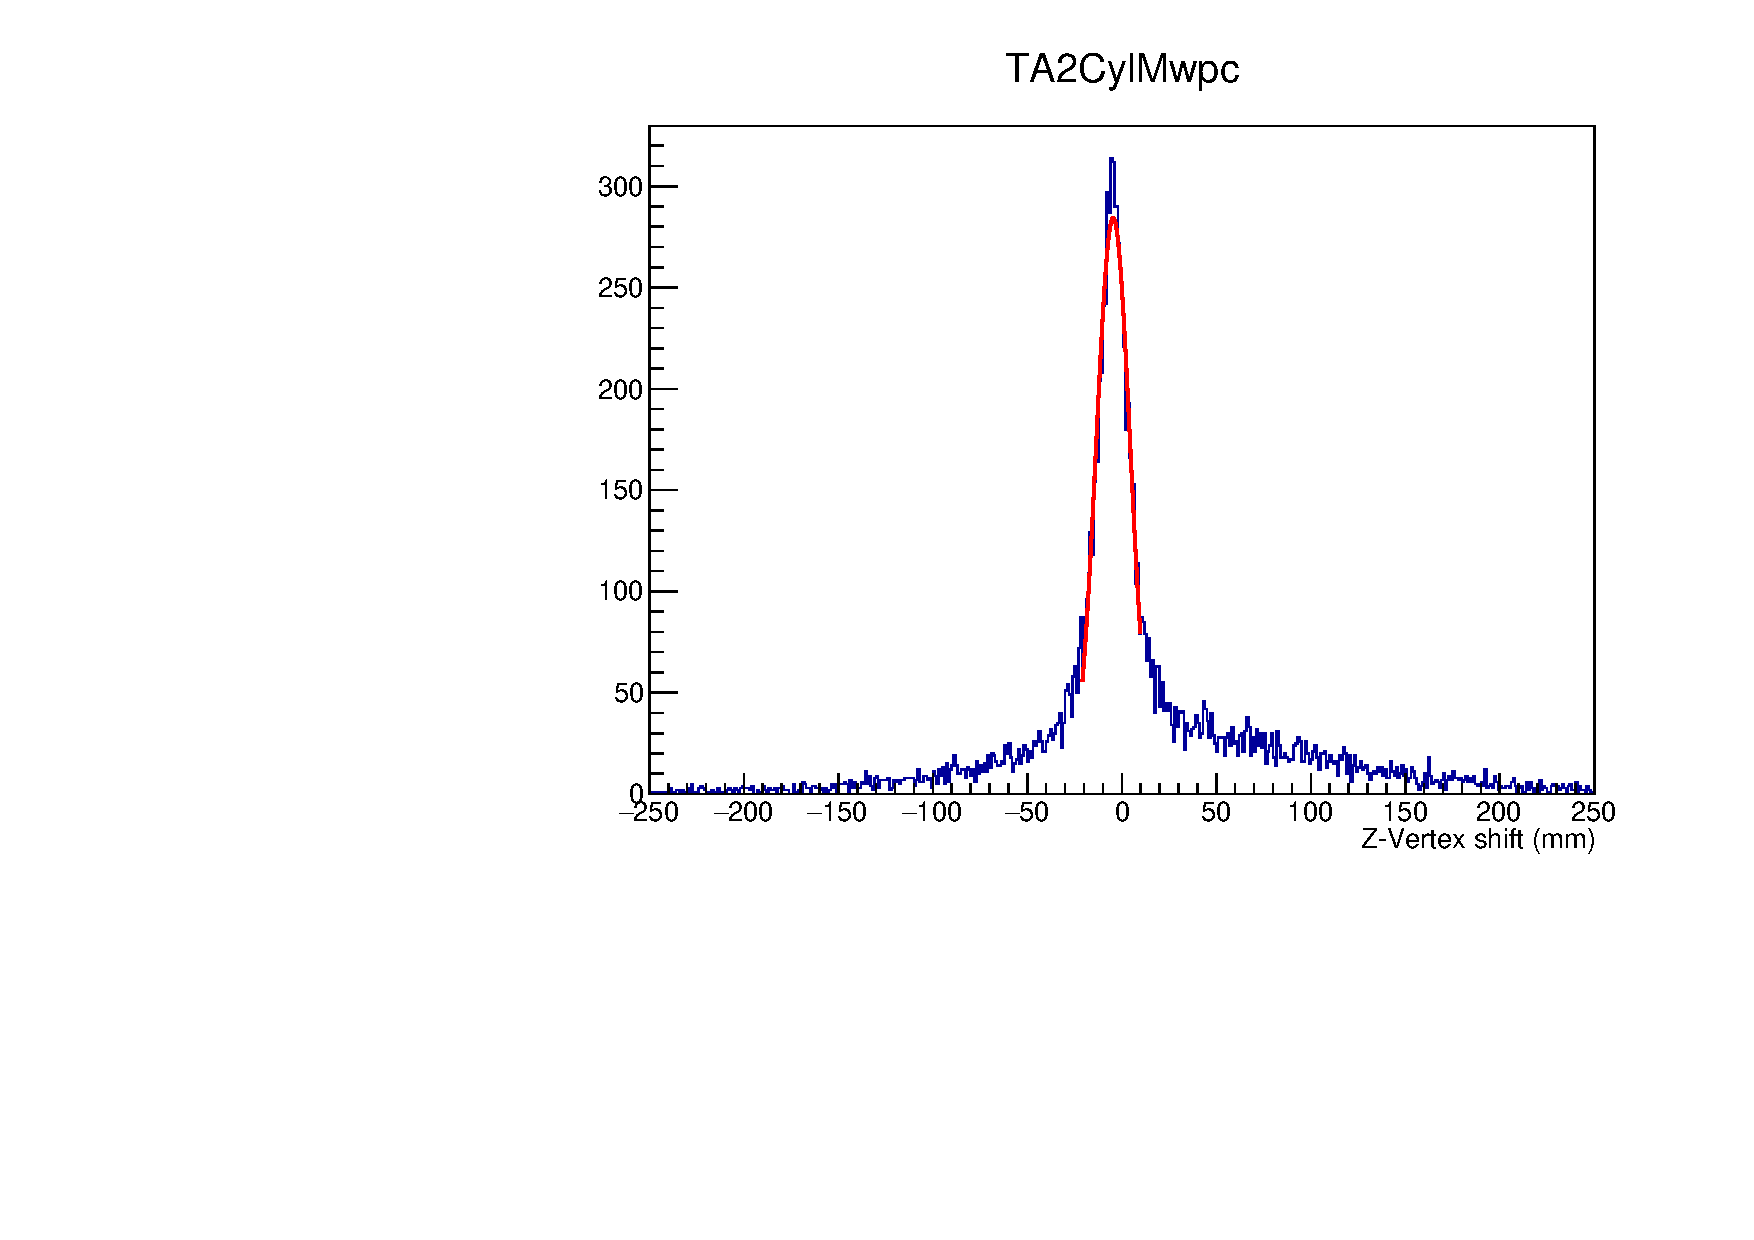
\includegraphics[scale=0.55]{pictures/pdf/VertexZ_sn116.pdf}
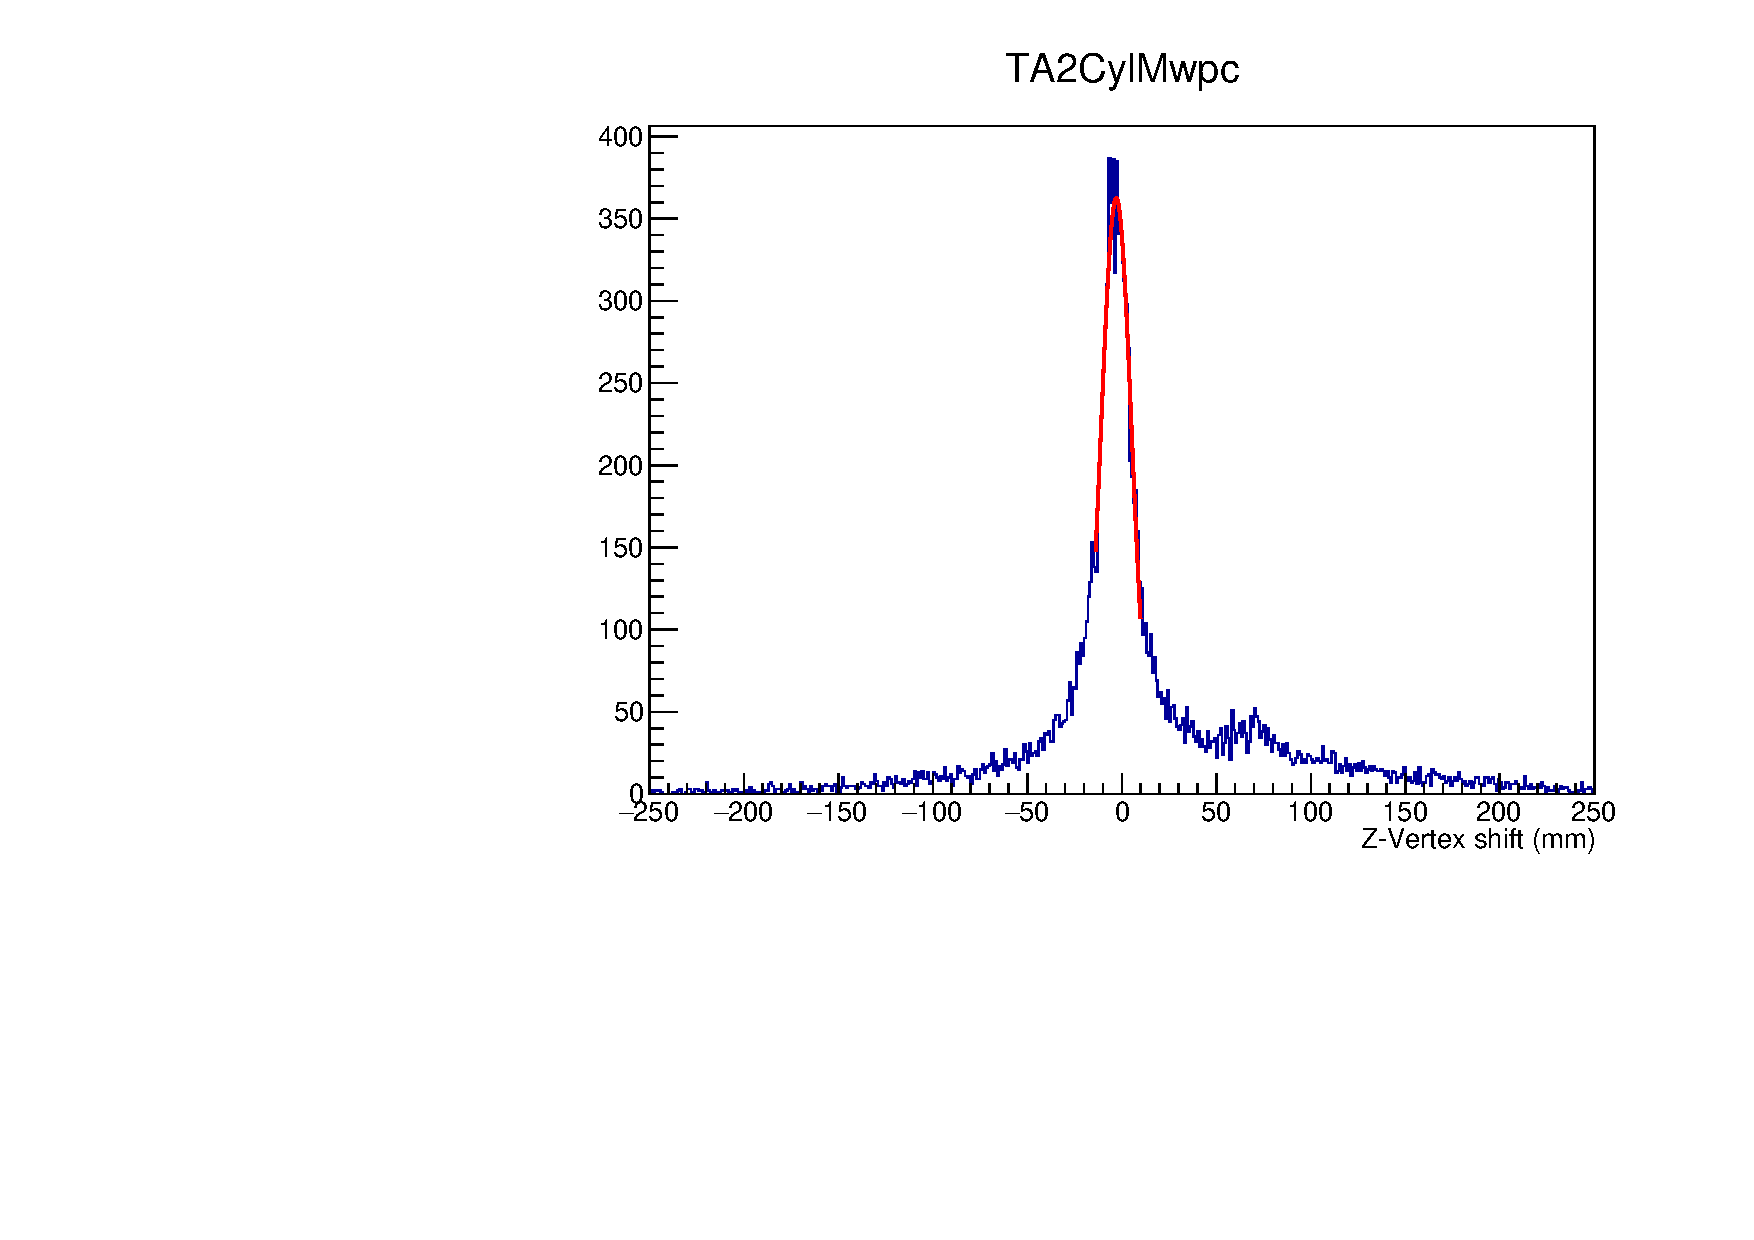
\includegraphics[scale=0.55]{pictures/pdf/VertexZ_sn120.pdf}
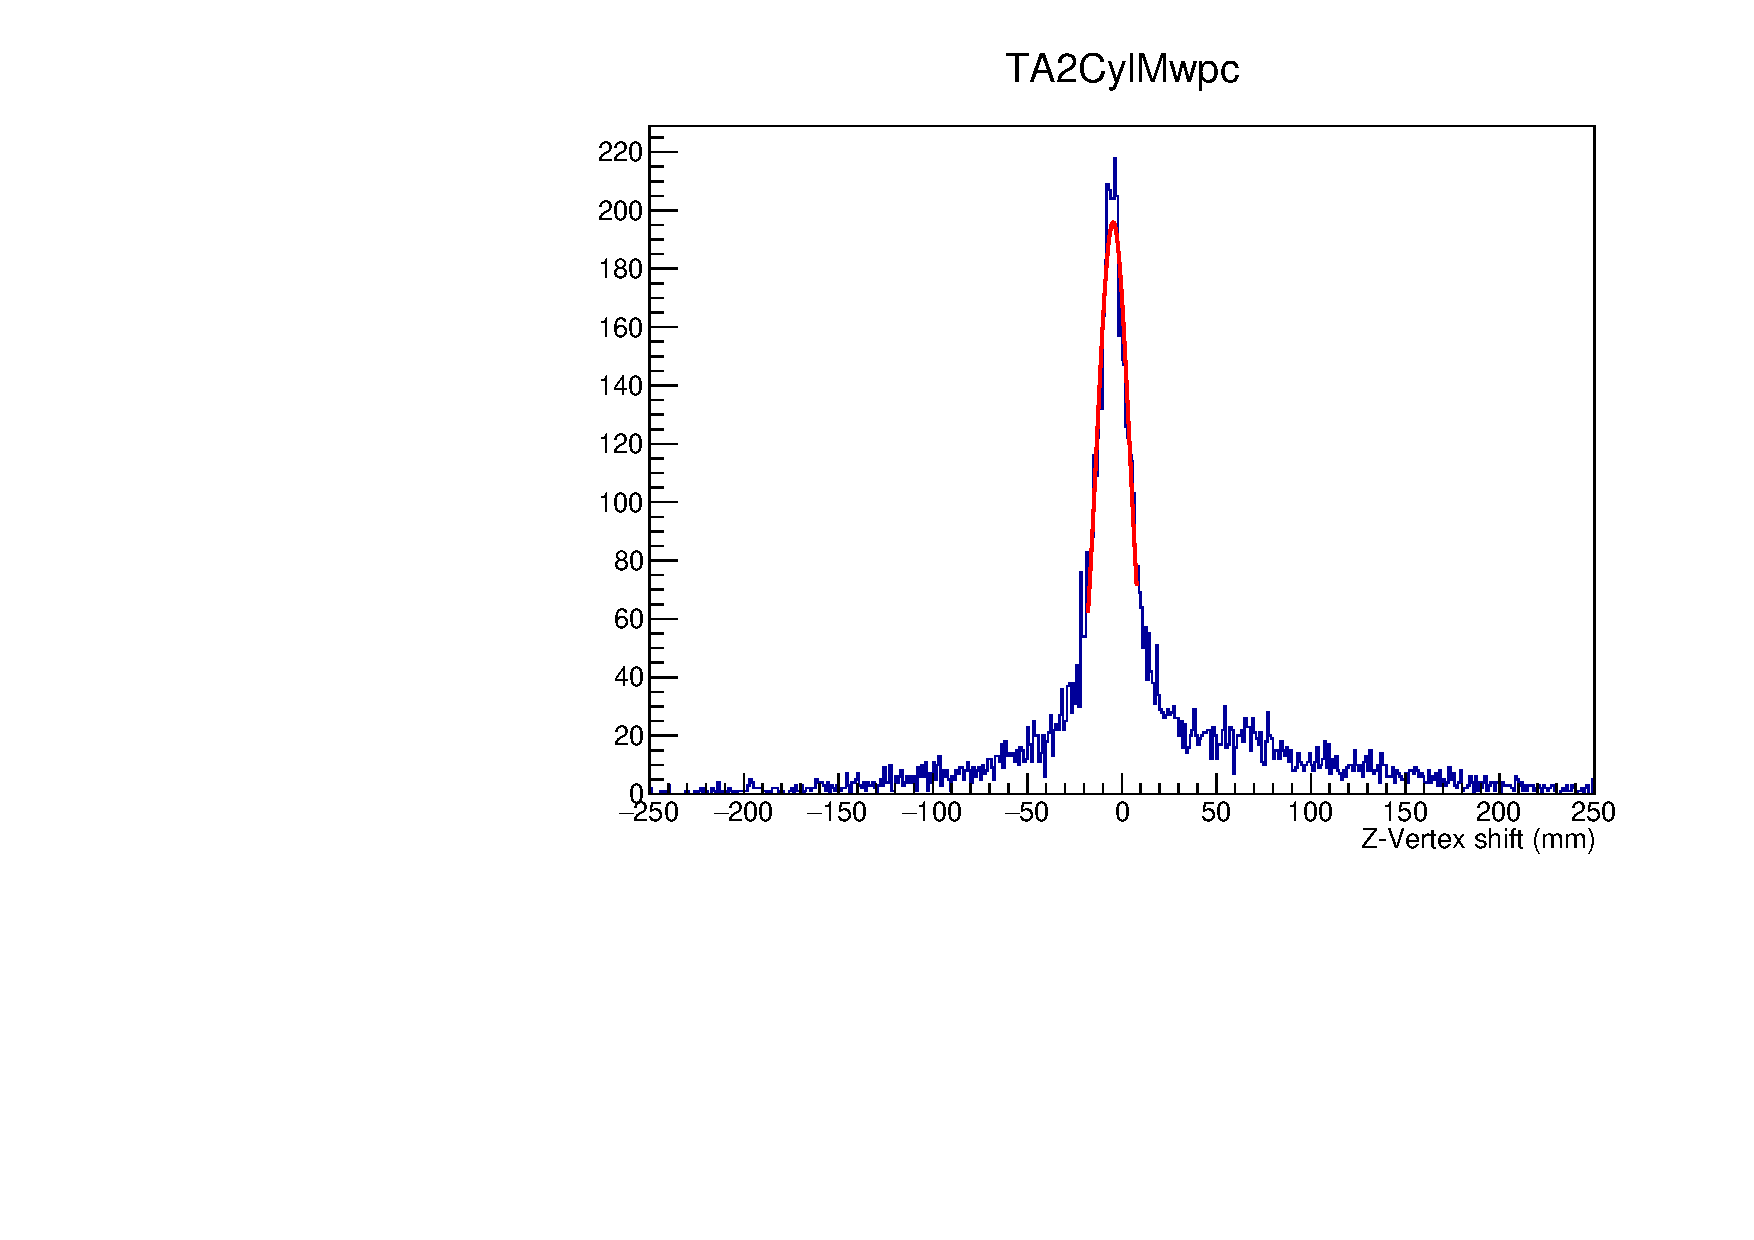
\includegraphics[scale=0.55]{pictures/pdf/VertexZ_sn124.pdf}
\caption{Target positioning. Top graph shows the fit results for the correction for $^{116}Sn$, middle grpah shows data for $^{120}Sn$, and the bottom graph shows the fitted offset for $^{124}Sn$.}
\label{targetvertex}
\end{center}
\end{figure}

The position of the target has been determined with the use of a Gaussian fit to the charged particle reaction vertices (Fig. \ref{targetvertex}). The mean of the Gaussian fit have been extracted and its value employed in the analysis as the target position correction.

\indent The obtained value of the position offset with respect to the Crystal Ball have been used in the analysis code to correct the momenta of the detected particles. The below formulas show how the momentum is calculated for the target located in the centre of the Crystal Ball (Equation \ref{mom1}) and how the calculation is corrected when the effect of the position offset is included (Equation \ref{mom2}):

\begin{equation}
p = \frac{E_{meas}}{\sqrt{x^{2}+y^{2}+z^{2}}}(x,y,z)
\label{mom1}
\end{equation}
\begin{equation}
p = \frac{E_{meas}}{\sqrt{x^{2}+y^{2}+(z-z_{corr})^{2}}}(x,y,z-z_{corr})
\label{mom2}
\end{equation}
where, $E_{meas}$ is the measured energy of the deposit in the cluster, $x$, $y$, and $z$ are the coordinates of the centre of mass of the cluster and $z_{corr}$ is the correction due to the target position offset determined with the MWPCs.

\indent The correction of the target z-vertex position has a direct effect on the calculations of reconstructed $\pi^{0}$ scattering angle $\theta$. By default, the event reconstruction assums that the target position is exactly at the centre of the Crystal Ball, including the target position correction shifts the reaction vertex upstream and gives more accurate calculations of the reconstructed pion scattering angle.

\section{Coherent Events}

\indent As described in chapter 2, the $\pi^{0}$ photoproduction can occur in several of ways, and alongside the coherent process, incoherent and quasi-free reactions take place. In order to extract the coherent events from the background, missing energy analysis has been performed. This technique uses information on incident photon energy from the tagger and $\pi^{0}$ 4-momentum reconstructed from the information recorded in the Crystal Ball.

\indent The pion missing energy is calculated with the following formula:

\begin{equation}
\Delta E_{\pi} = E_{\pi}^{CoM}(E_{\gamma})-E_{\pi}^{CoM}(E_{\gamma_{1}\gamma_{2}})
\end{equation}
where $E_{\pi}^{CoM}(E_{\gamma})$, defined in equation \ref{pienergy} is the pion energy in the pion-nucleus centre of mass frame of reference. $E_{\gamma}$ in the incident photon energy, $s$ is the invariant mass of the photon-nucleus system and $m_{\pi}$and $M^{2}$ are the masses of pion  and the nucleus respectively. $E_{\pi}^{CoM}(E_{\gamma_{1}\gamma_{2}})$ is the, Lorentz-transformed to the CoM reference frame, detected pion energy.

\begin{equation}
E_{\pi}^{CoM}(E_{\gamma})=\frac{s+m_{\pi}^{2}-M^{2}}{2\sqrt{s}}
\label{pienergy}
\end{equation}

\indent Although the pion energy can be approximated as the sum of the energies of the two decay photons, considering the angular information of the reaction allows for much better energy resolution, and therefore, more accurate calculations \cite{miller}:

\begin{equation}
E_{\pi} = \sqrt{\frac{2m_{\pi}^{2}}{(1-\frac{E_{1}-E_{2}}{E_{1}+E_{2}}^{2})(1-cos\phi)}}
\end{equation}
where, $E_{1}$ and $E_{2}$ are the detected energies of the two decay photons and $\phi$ is the opening angle between them. The Lorentz transformation of the detected pion energy to the CoM frame of reference is calculated with:

\begin{equation}
E_{\pi}^{CoM} = \gamma\Big(E_{\pi}-\frac{E_{\gamma}}{E_{\gamma}+M}\big(E_{1}cos\theta_{1}+E_{2}cos\theta_{2}\big)\Big)
\end{equation}
where, $\theta_{1}$ and $\theta_{2}$ are the polar angles of the two decay photons, $E_{\pi}$ is the detected pion energy.

\indent The condition for the coherent $\pi^{0}$ photoproduction process is satisfied when $E_{\pi}^{CoM}(E_{\gamma})$ and $E_{\pi}^{CoM}(E_{\gamma_{1}\gamma_{2}})$ are the same. Background processes however, return negative values of $\Delta E_{pi}$ since the initial energy is split between other than $\pi^{0}$ particles produced in the reaction or used up to promote the nucleus to an excited state.

\indent In order to extract the coherent $\pi^{0}$ yield the missing energy spectrum has been split into several energy bins in the photon energy range from 135 to 580 $MeV$, and initially into 180 angular bins in the $\theta_{\pi}$ range of $0-180^{\circ}$. The resulting spectra were then fitted with one or two functions describing the coherent and background signals.

\indent The fitting procedure has benefited greatly from the existing knowledge about eleastic and inelastic cross sections. In the electron scattering experiments it has been already shown that elastic form factors peaks in the forward direction \cite{isick}, from there it follows that the elastic cross sections will be forward peaked as well. For the incoherent processes, however, the form factor and so the cross section variation is much smaller across the pion scattering angular range \cite{takaki}. This behaviour implies that for the coherent $\pi^{0}$ scattering regions, the $\Delta E_{\pi}$ spectrum will be entirely dominated by the coherent peak. This should allow to fit the coherent peak and determine its fit parameters with a high level of confidence. This fit information can be subsequently used for the fits in the regions where incoherent contributions dominate.

\indent The first step in the fitting procedure was plotting the 2D spectra of pion scattering angle. $\theta_{\pi}$ against the pion missing energy, $\Delta E_{\pi}$ for the photon energies in the range of $E_{\gamma} = 135 - 580 MeV$, an exmaple plot is shown in Fig. \ref{2drandomsub}.

\begin{figure}[H]
\begin{center}
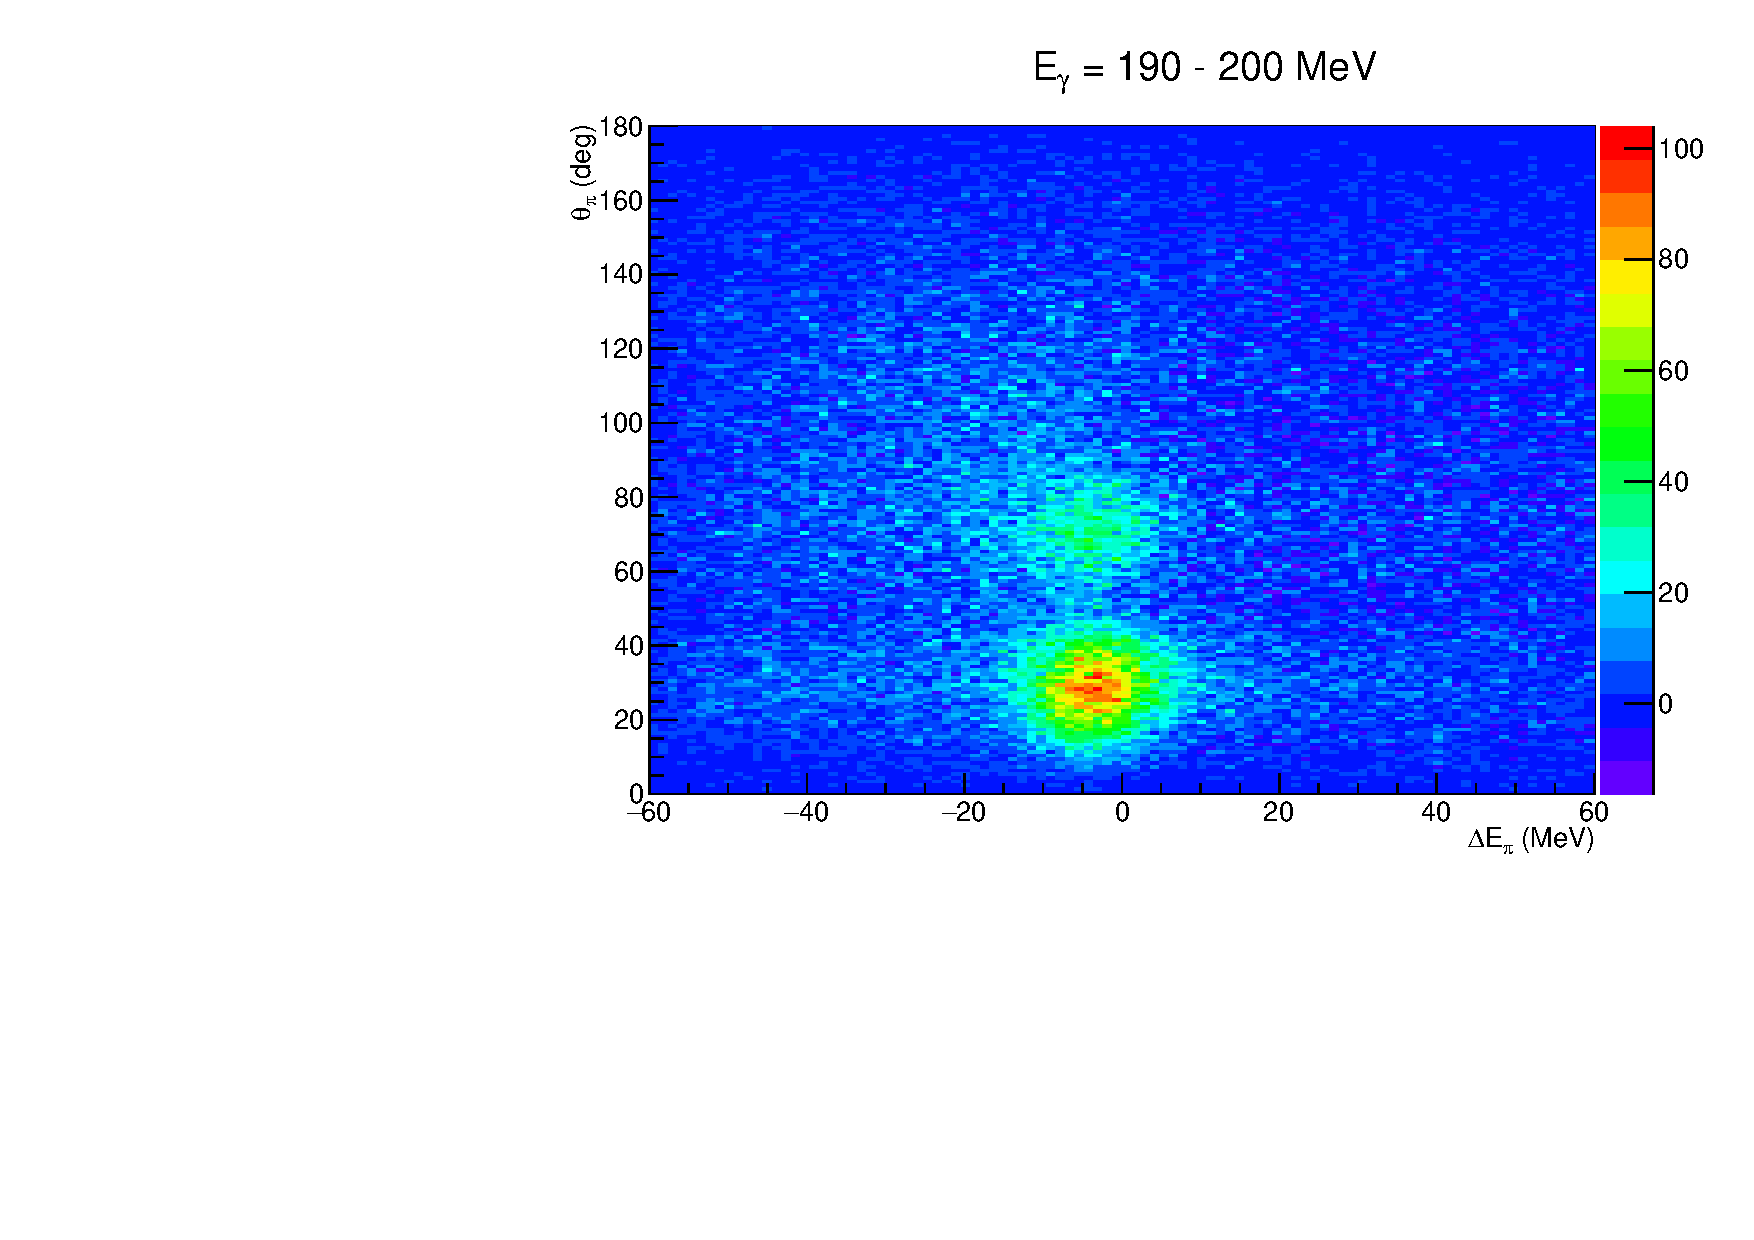
\includegraphics[scale=0.65]{pictures/pdf/2d_sn116_eg7.pdf}
\caption{The plot of the pion scattering angle $\theta_{\pi}$ agains pion missing energy $\Delta E_{\pi}$ for the $^{116}Sn$ data.}
\label{2drandomsub}
\end{center}
\end{figure}

\indent Next, the 2D spectra have been projected along the x-axis in $3^{\circ}$ angular bins creating an array of one dimensional histograms. Then, nine projections around the first diffraction maximum (the angular range of $15-36^{\circ}$) have been selected to fit the coherent signal with a Gaussian function. The width of the fit have been extracted and using this values to constrain the coherent peak a second iteration of fits has been performed. This time however, a fit function built from to Gaussian functions have been used to fit the data. The below figure shows the fits around the diffraction maximum and minimum.

\indent The area of the Gaussian function fitted to the coherent peak has been also calculated and stored as a measure of the coherent yield of the reaction \cite{claire2}.

\begin{figure}[H]
\begin{center}
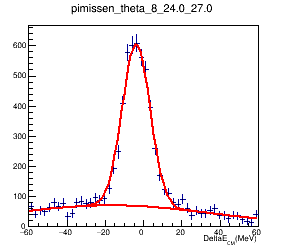
\includegraphics[scale=0.65]{pictures/png/fit_coherent.png}
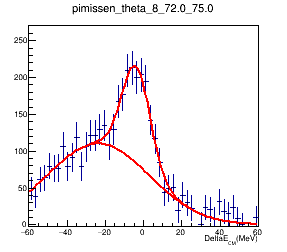
\includegraphics[scale=0.65]{pictures/png/fit_incoherent.png}
\caption{The fits to the pion missing energy spectrum for the energy bin $E_{\gamma} = 200 MeV$. The graph on the left shows the fit around the first diffraction maximum, and the graph on the right shows the fit around the diffraction minimum.}
\end{center}
\end{figure}

\indent The below plot shows the pion missing energy spectra after the background subtraction.

\begin{figure}[H]
\begin{center}
%\includegraphics[scale=0.65]{pictures/pdf/.pdf}
\caption{The plot of the pion scattering angle $\theta_{\pi}$ agains pion missing energy $\Delta E_{\pi}$ for the $^{116}Sn$ data after the background subtraction.}
\label{2dbackgroundsub}
\end{center}
\end{figure}


\section{Tagging Efficiency}

\indent A tagging efficiency measurements have been performed in order to accurately determine the beam luminosity, which is necessary for the $pi^{0}$ yield normalisation in the cross section measurements. As described in chapter 3, the information about the photon flux is obtained from the number of hits in the FP detector. However, when the beam passes through the collimator further photons are removed form it and in order to account for this reduction in the flux a dedicated measurement with a lower beam intensity is performed.

\indent The measurements have been taken for each target separately and the results are presented in the below figure (Fig. \ref{taggingeff}).

\begin{figure}[H]
\begin{center}
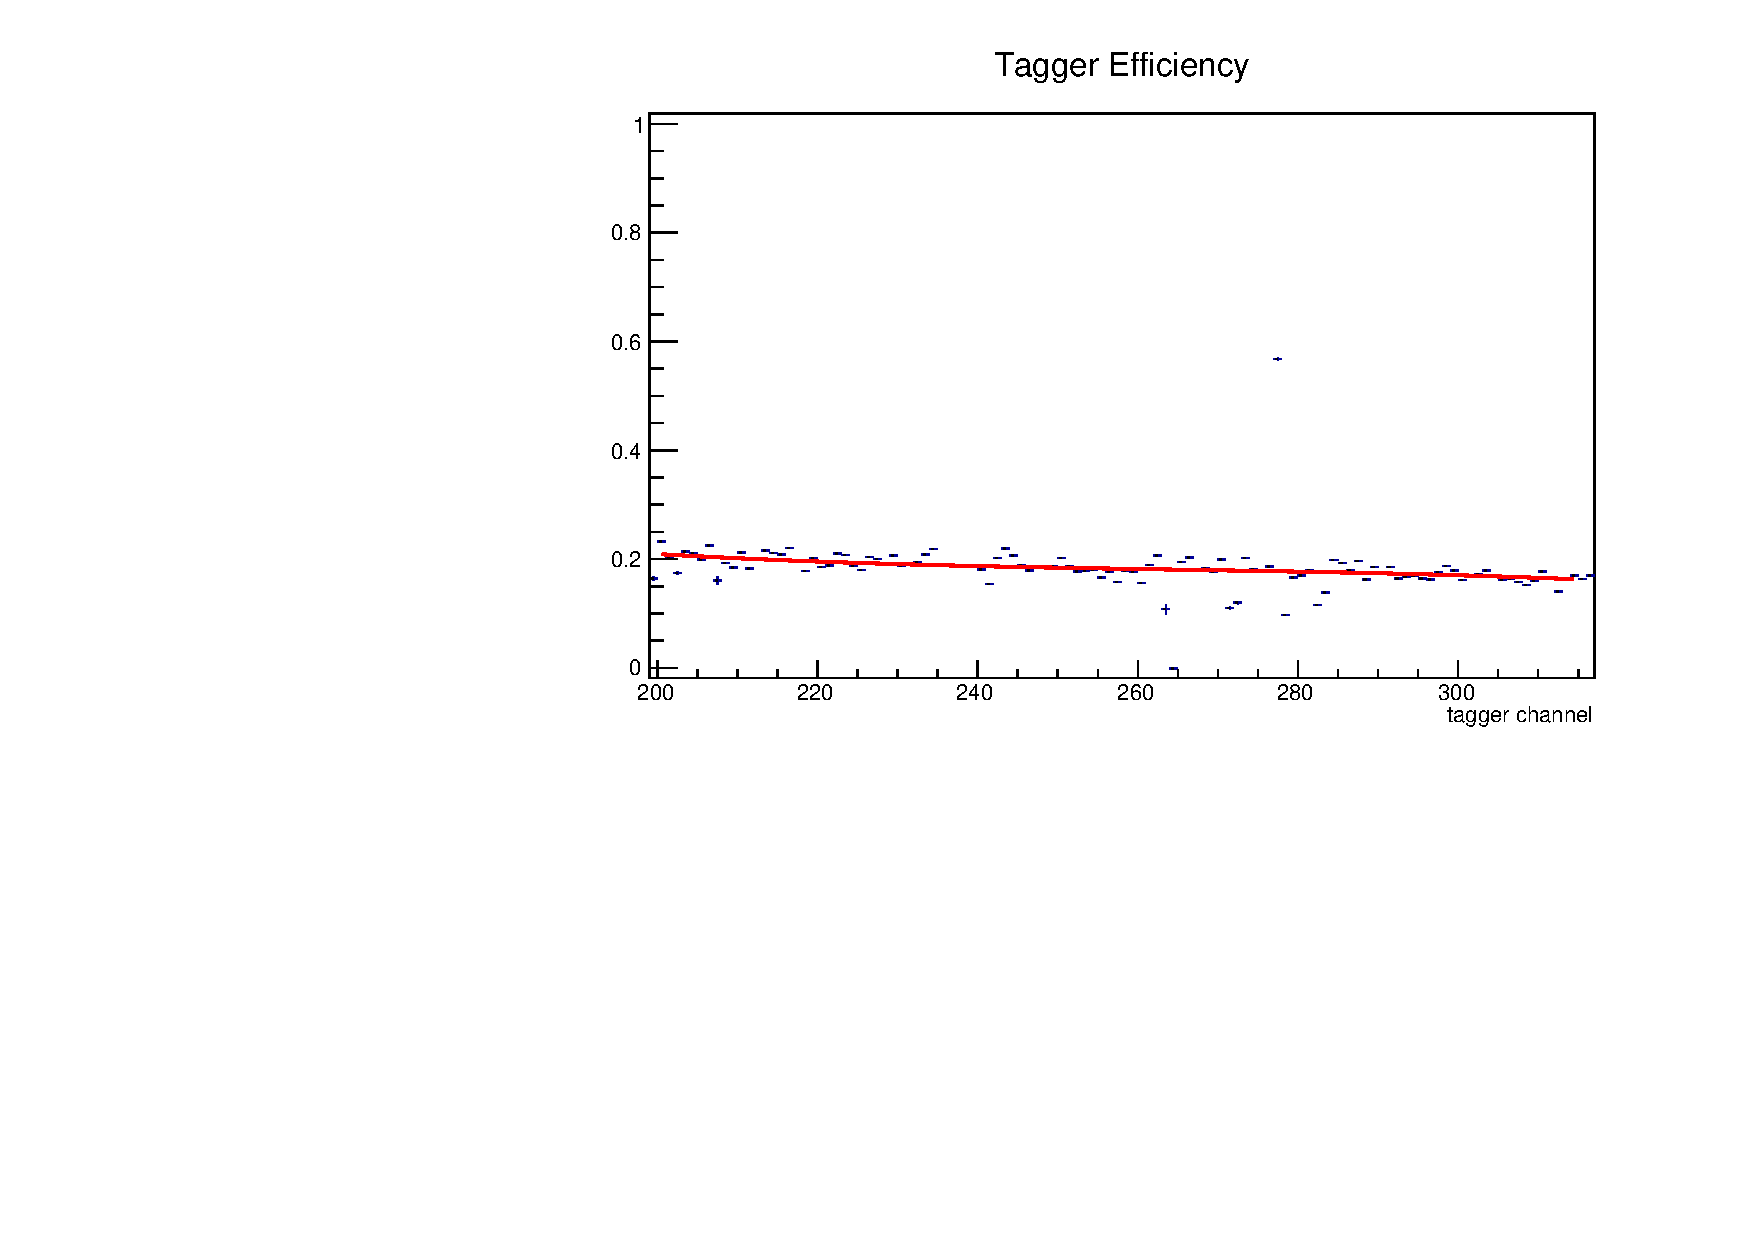
\includegraphics[scale=0.55]{pictures/pdf/tagging_efficiency_Sn116.pdf}
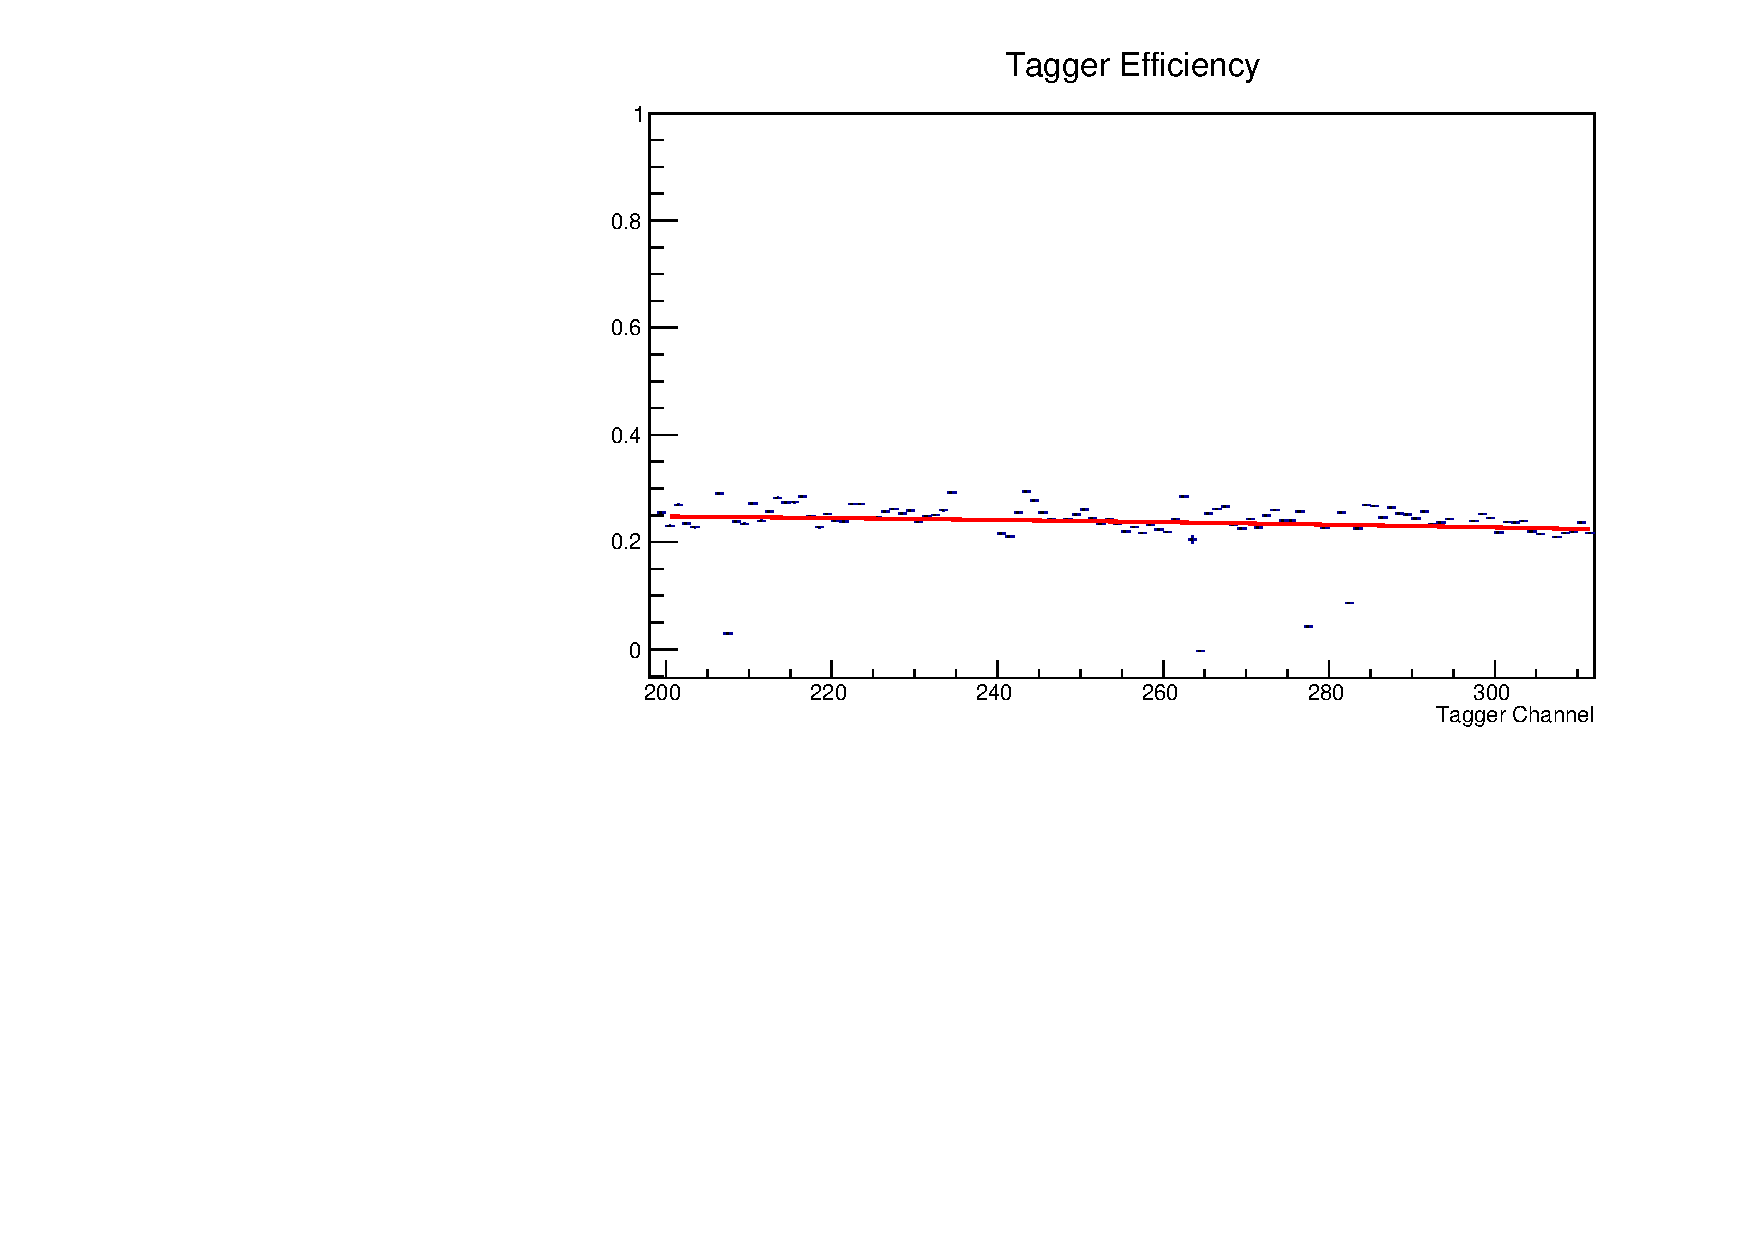
\includegraphics[scale=0.55]{pictures/pdf/tagging_efficiency_Sn120.pdf}
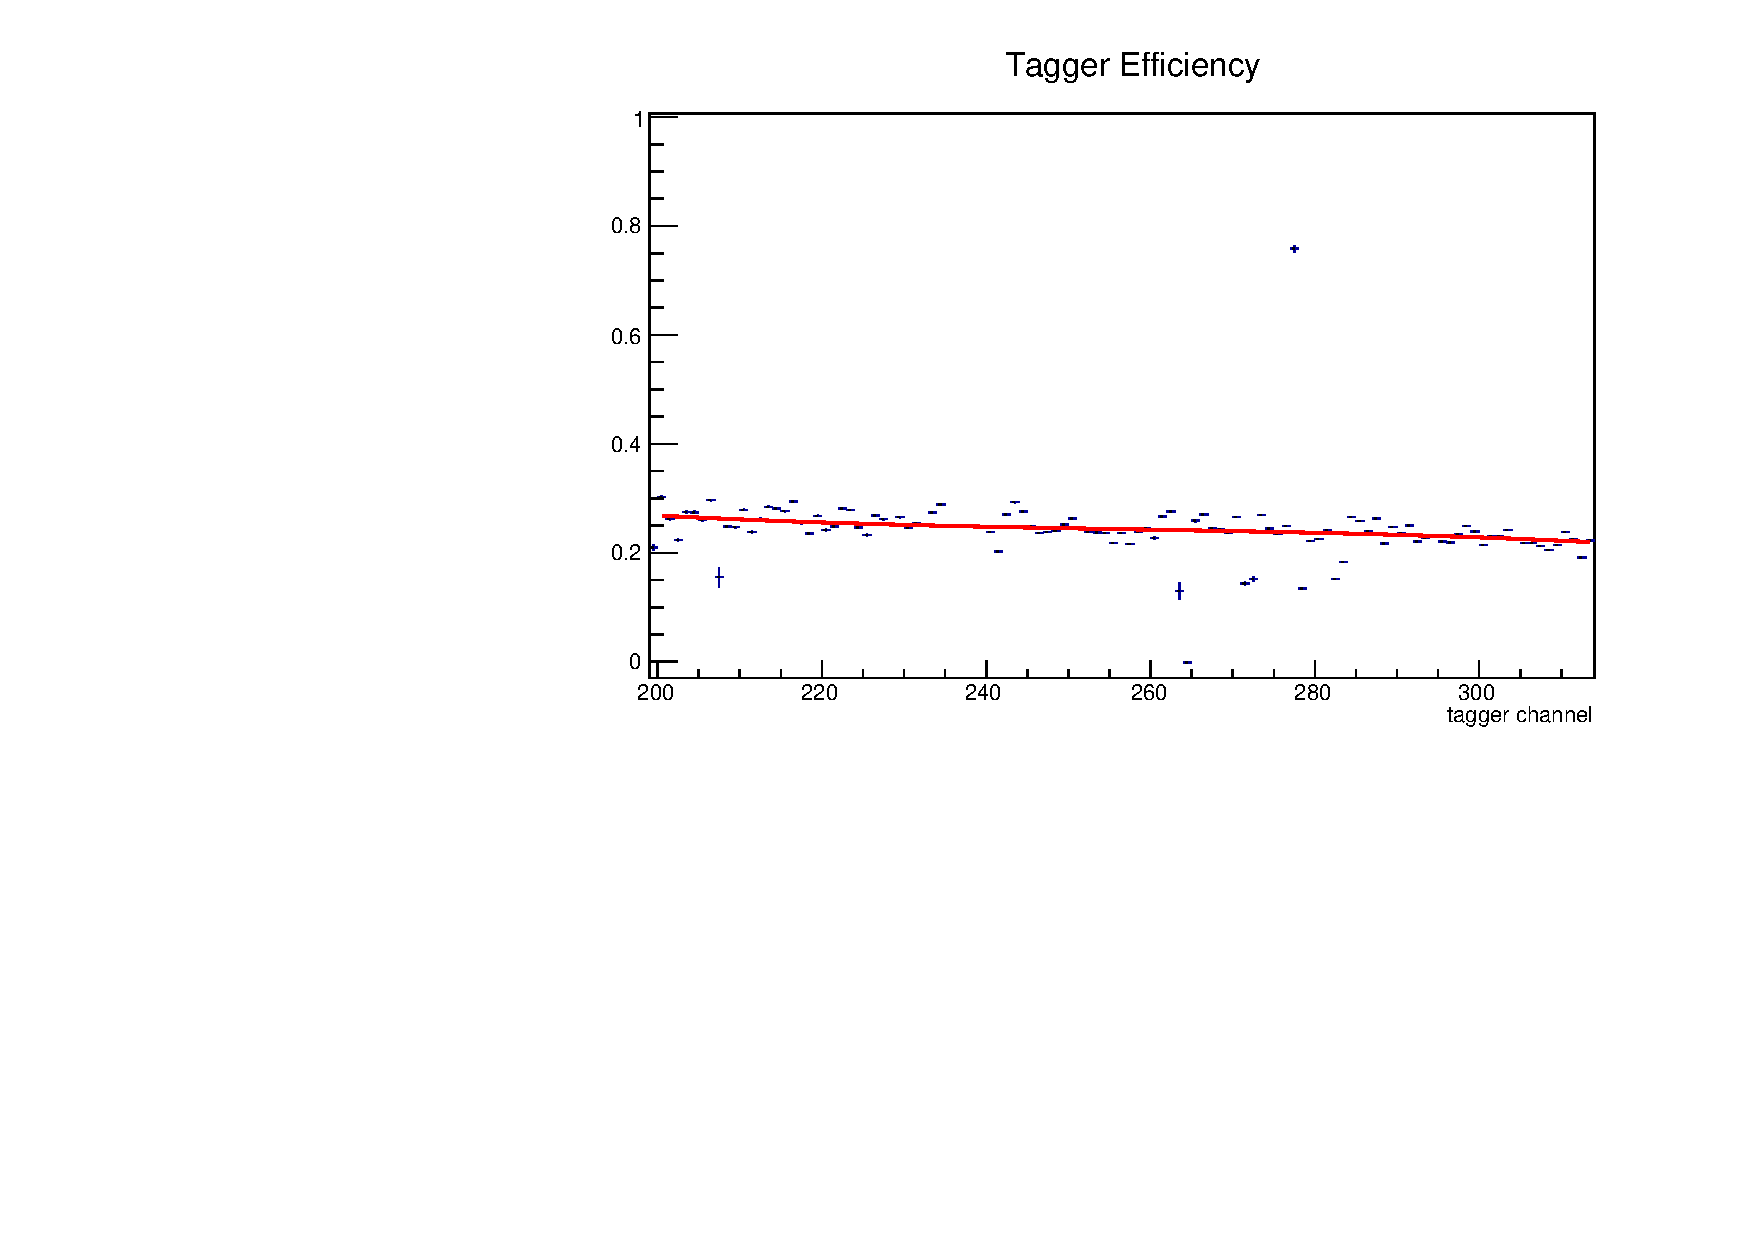
\includegraphics[scale=0.55]{pictures/pdf/tagging_efficiency_Sn124.pdf}
\caption{Tagging efficiency as a function of channel number for the tin targets. The top graph shows the results for $Sn^{116}$, the middle graph shows the results for $Sn^{120}$ and in the bottom graph are results for $Sn^{124}$.}
\label{taggingeff}
\end{center}
\end{figure}


\section{$\pi^{0}$ detection efficiency}

\indent A Geant4 Monte Carlo simulation has been used to calculate the efficiency of the detector setup.

\indent In order to decrease the time required for the simulation, the minimum number of the generated events have been decided upon. This number was based on the analysis of the impact on the total error on detection efficiency ($\epsilon_{det}$), which in turn depends on the error on generated and reconstructed events.

\indent It has been calculated that the error on the reconstructed events in the coherent peak was $\sim1\%$. Setting this value as the maximum error on detection efficiency, calculations to obtain a number of generated events such that the error on $\epsilon_{det}$ was no higher than the error due to reconstructed events have been done. They yielded a value of 10 millions.

\indent The $A(\gamma,\pi^{0})A$ events have been generated for the energy range of $135-540MeV$, for each target. Those generated events have then been used as the input of the Geant4 simulation. The resulting data have then been analysed with the same analysis software as the experimental data.

\indent The detection efficiency has been calculated for each energy and $\theta$ bin as the the ratio of the total number of detected $\pi^{0}$'s to the total number of $\pi^{0}$'s generated in that energy and $\theta$ bin.

\indent The dependence of the detection efficiency on the angle is shown in the below figures. The points at the edges don't follow the polynomial fit because the distribution fluctuates on both sides of the point at the poles and without introducing $\phi$ discrimination it is not possible to improve on this.

\begin{figure}[H]
\begin{center}
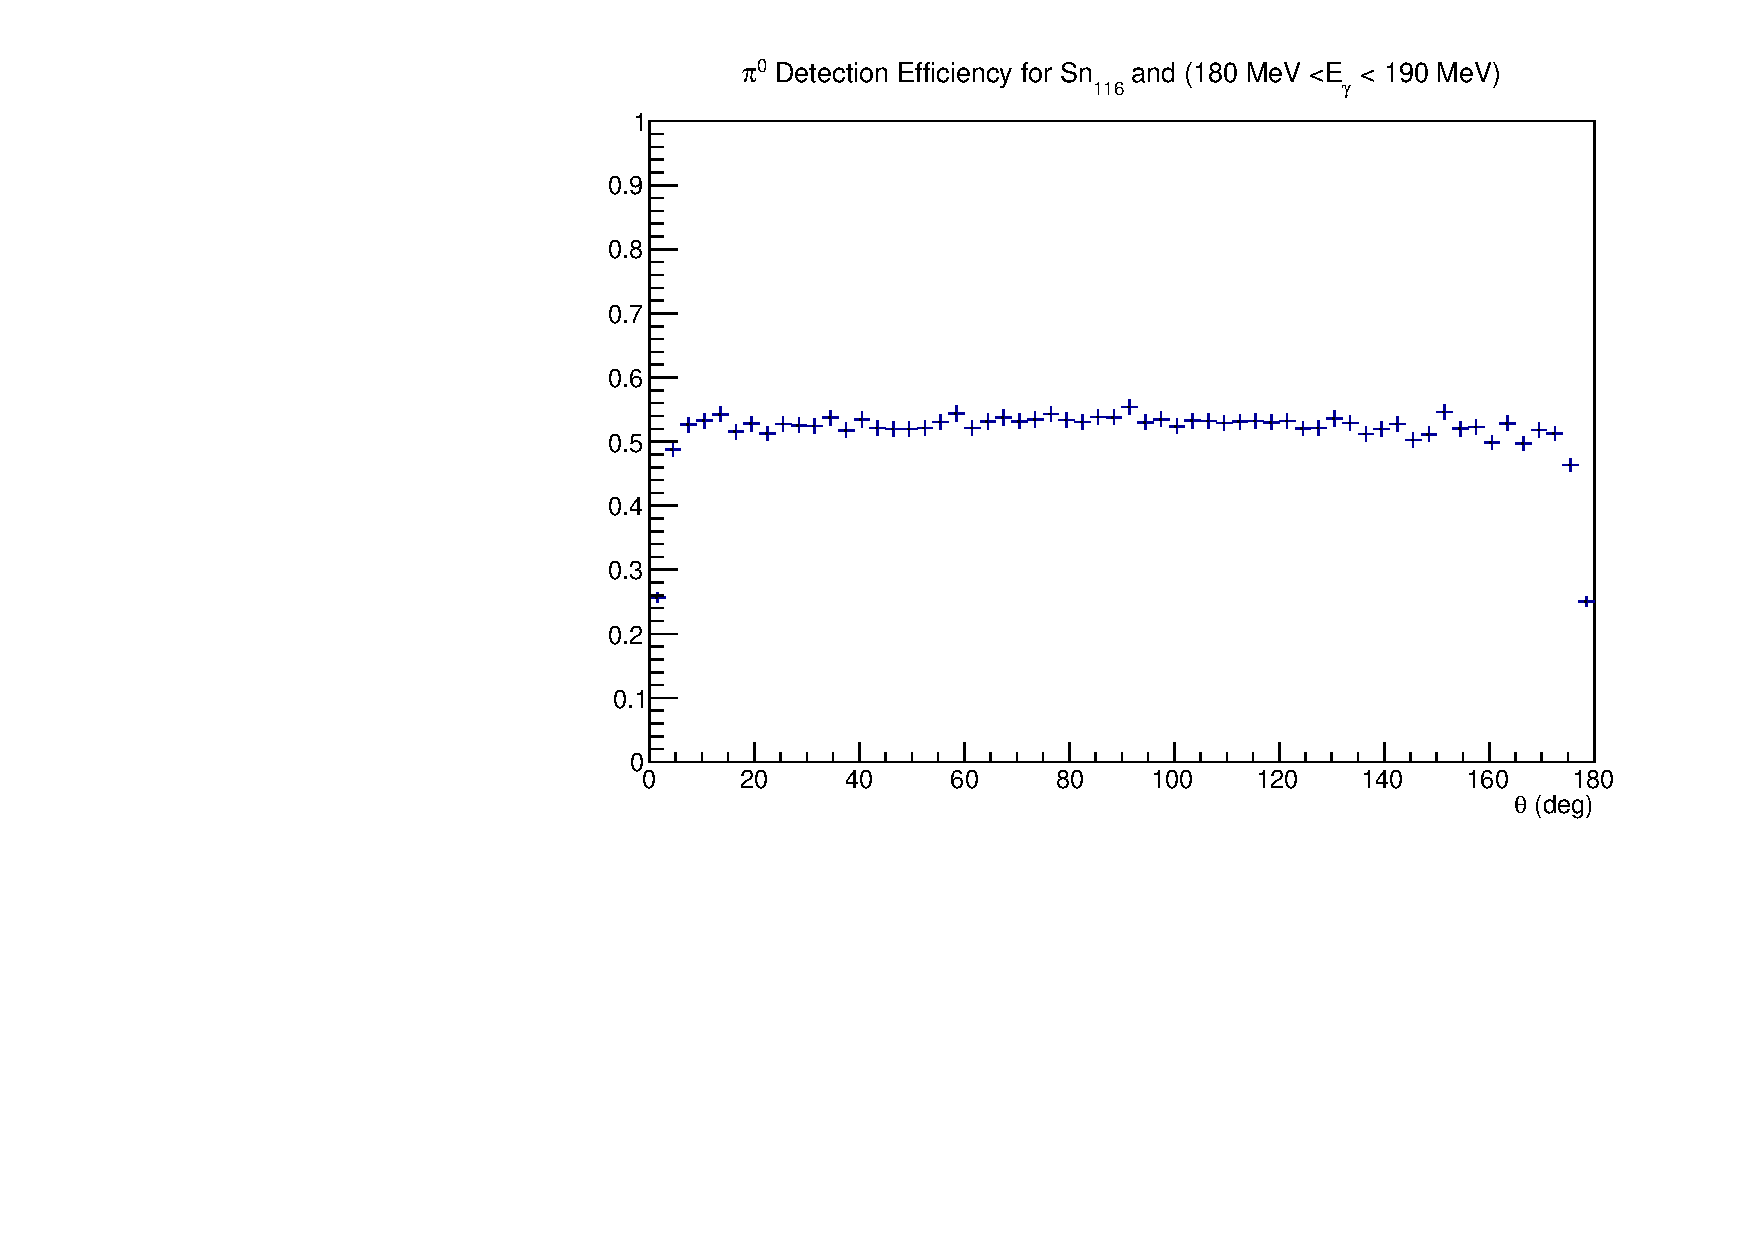
\includegraphics[scale=0.4]{pictures/pdf/pi0_efficiency_Sn116_Ebin6.pdf}
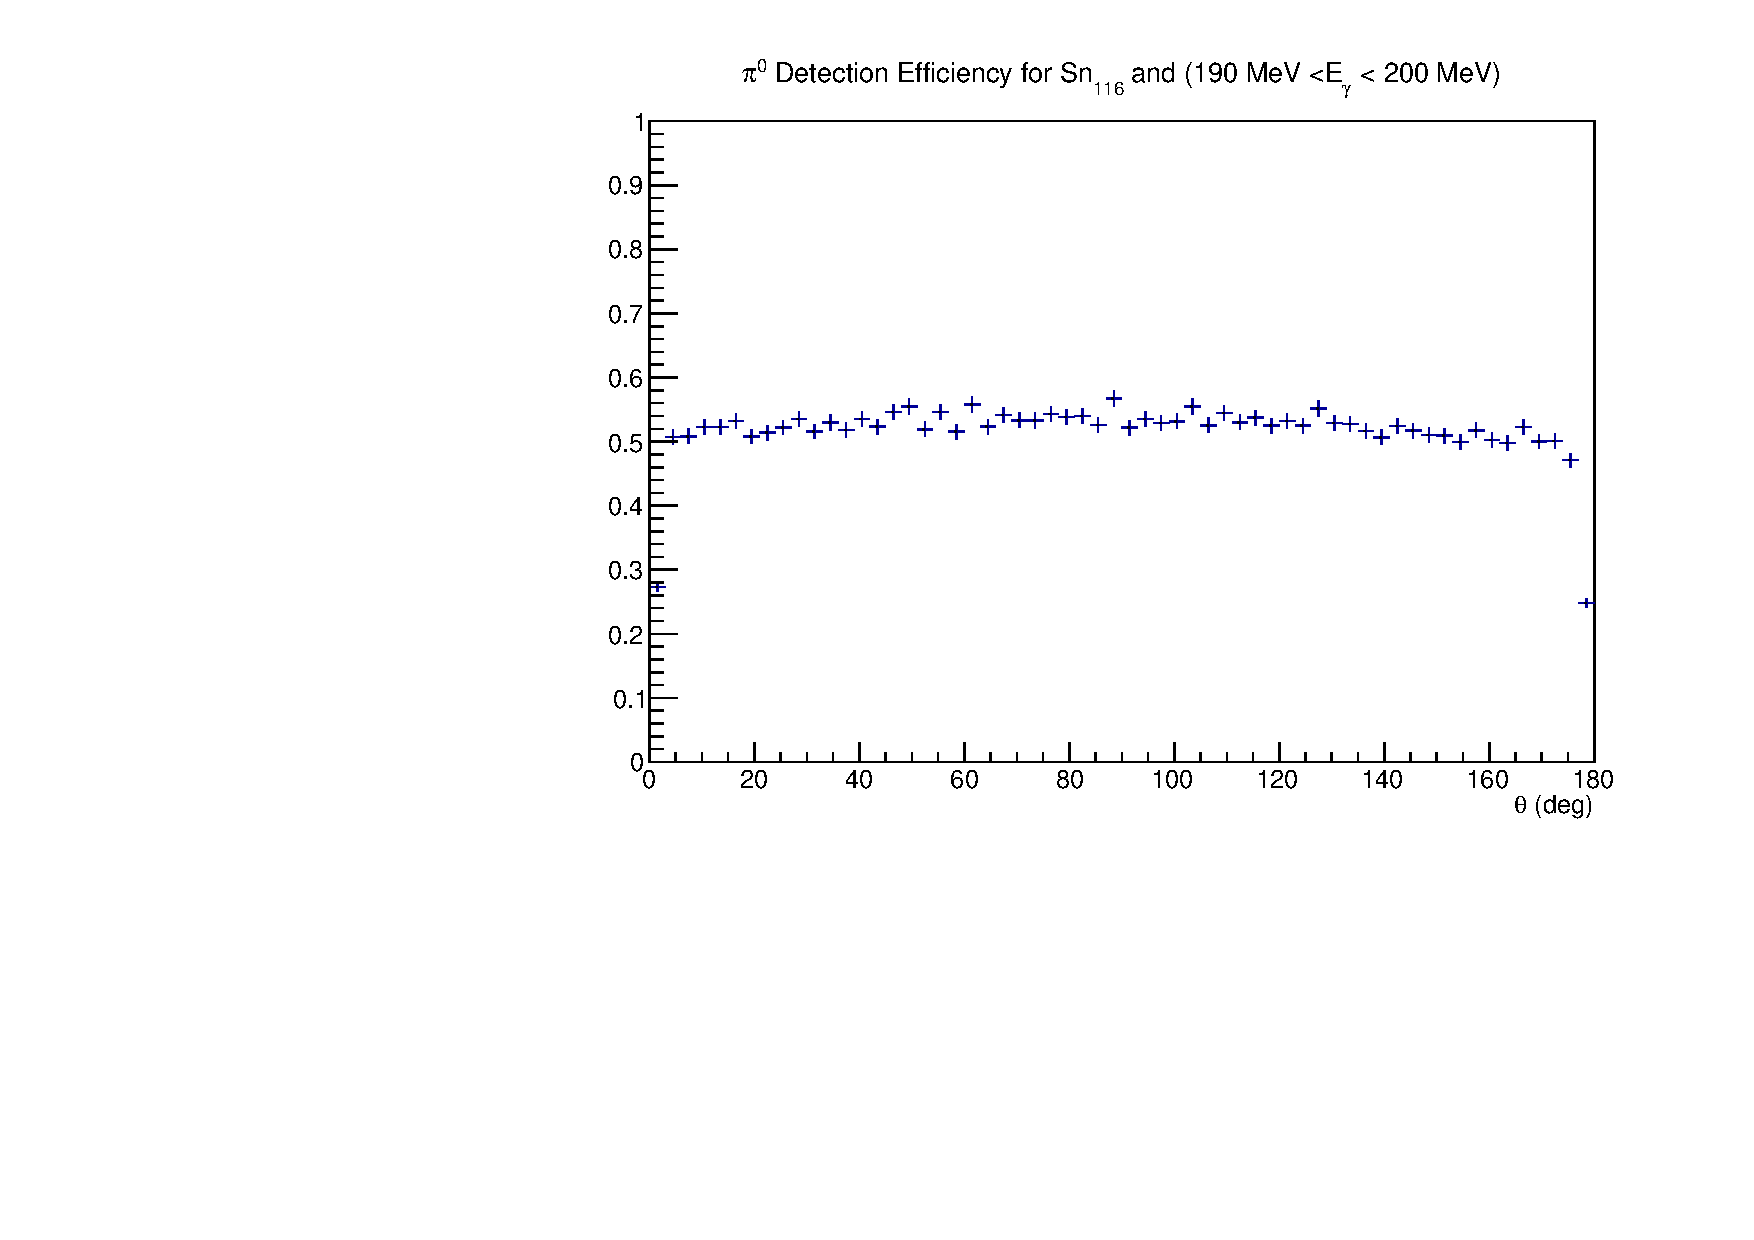
\includegraphics[scale=0.4]{pictures/pdf/pi0_efficiency_Sn116_Ebin7.pdf}
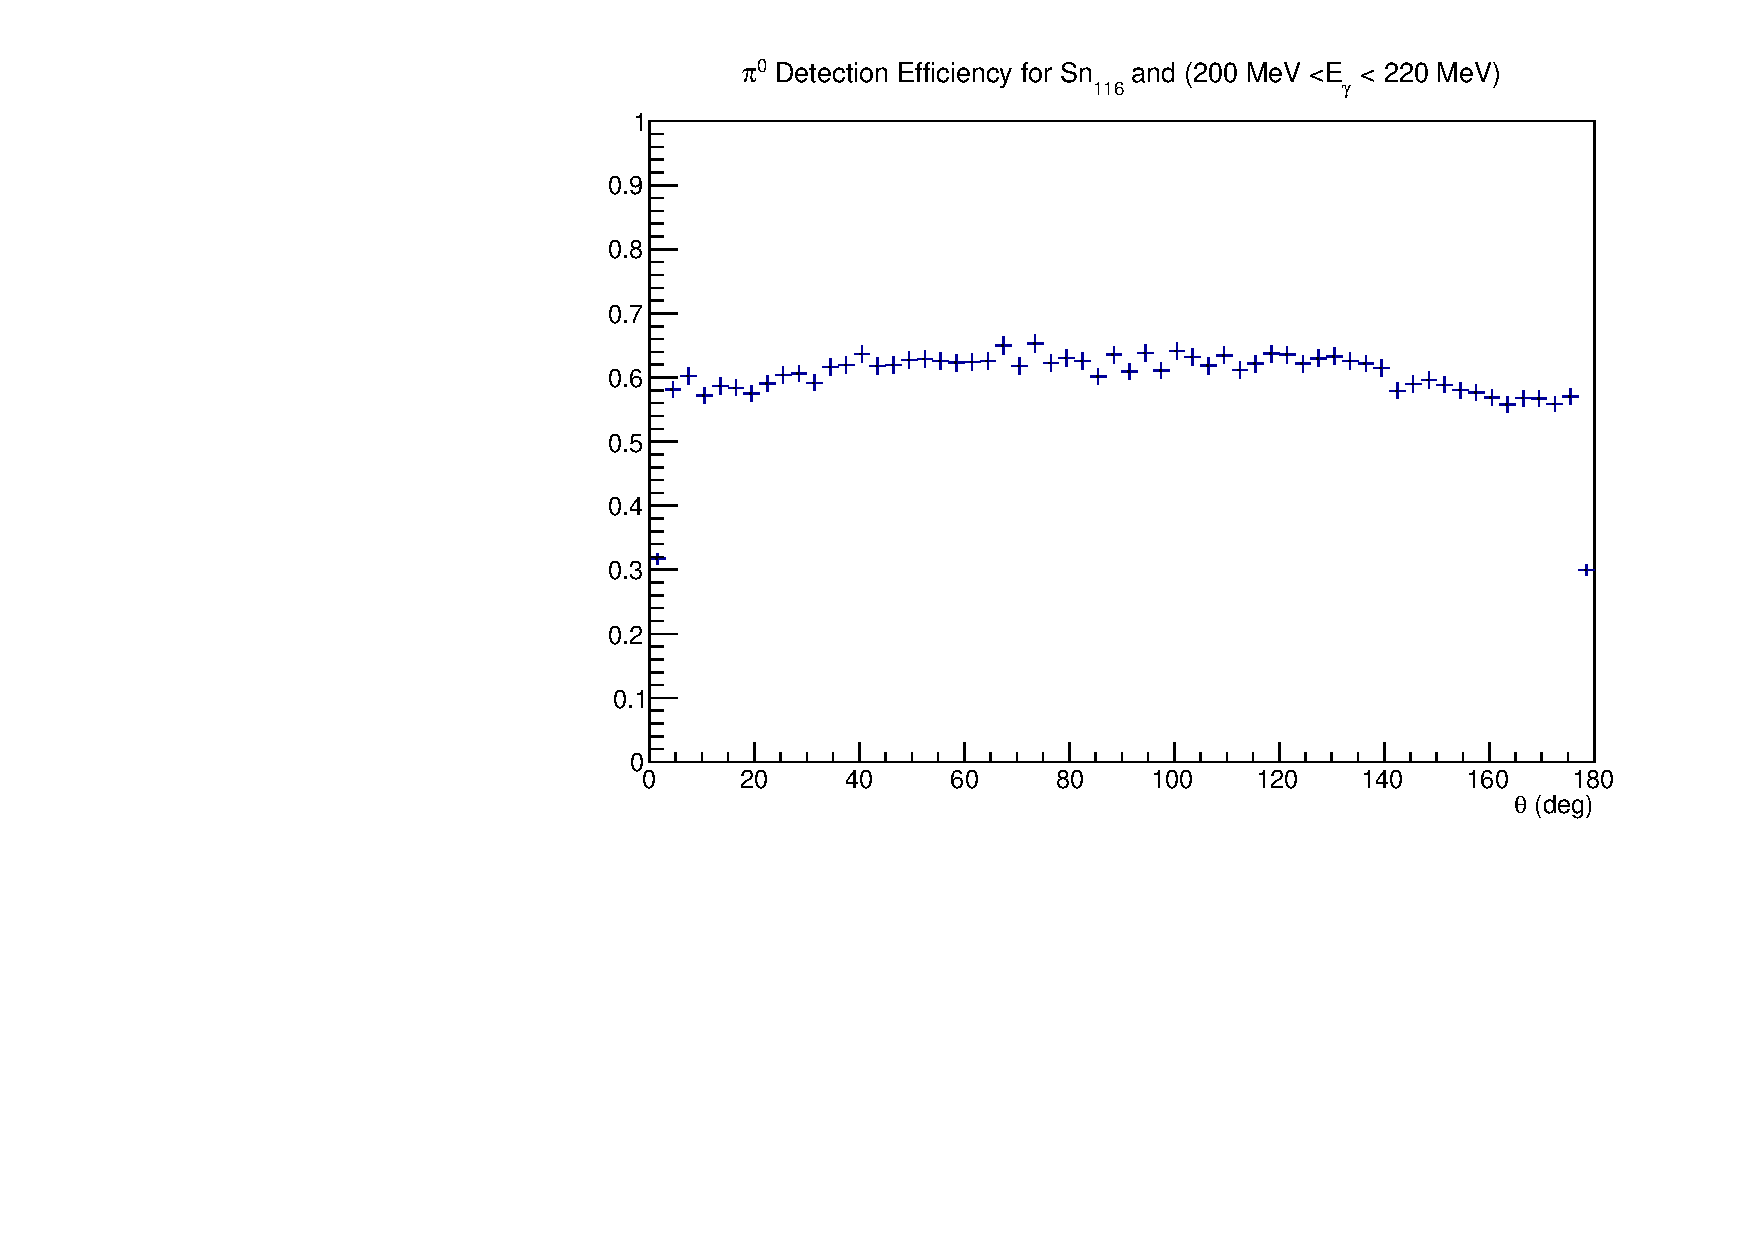
\includegraphics[scale=0.4]{pictures/pdf/pi0_efficiency_Sn116_Ebin8.pdf}
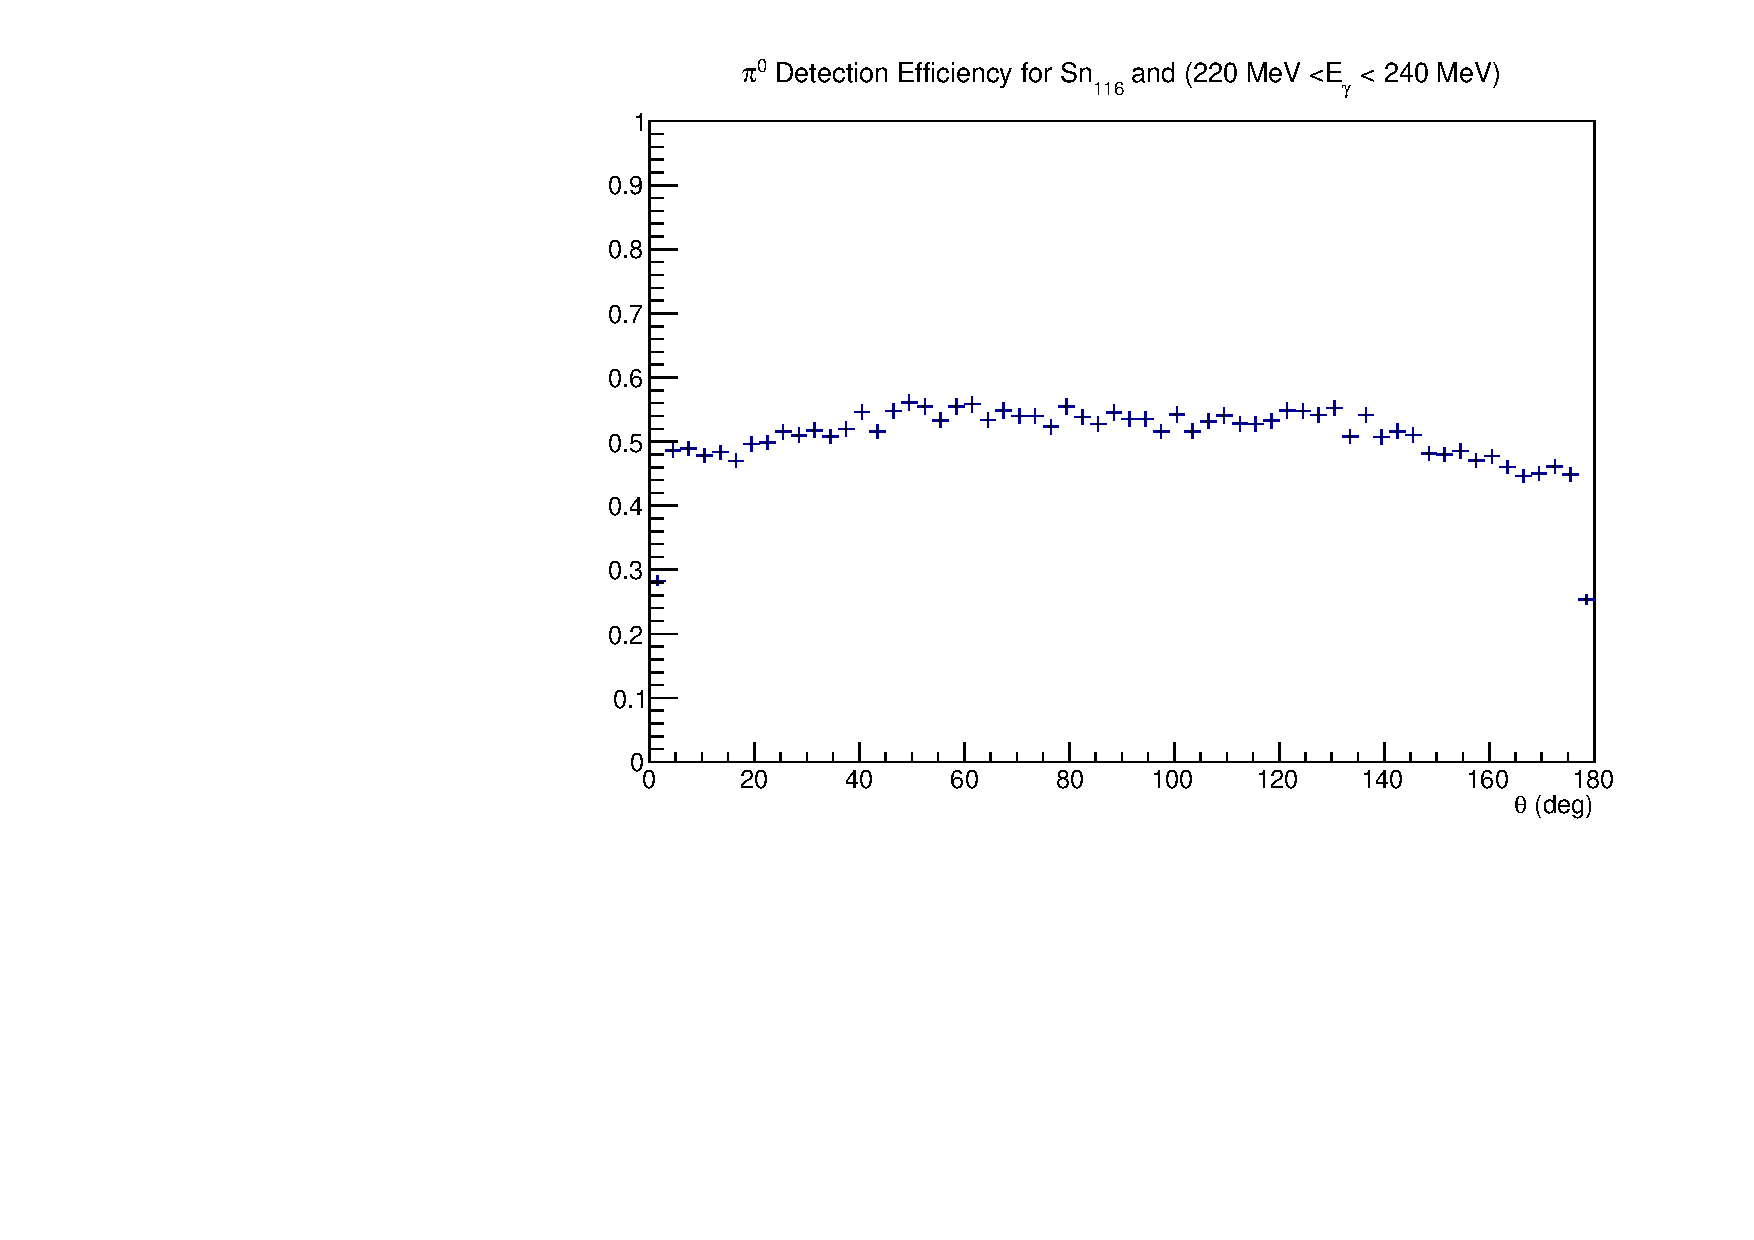
\includegraphics[scale=0.4]{pictures/pdf/pi0_efficiency_Sn116_Ebin9.pdf}
\caption{Dependence of the detection efficiency on energy and $\theta_{\pi^{0}}$ for the $^{116}Sn$ target.}
\label{detectioneff1}
\end{center}
\end{figure}

\begin{figure}[H]
\begin{center}
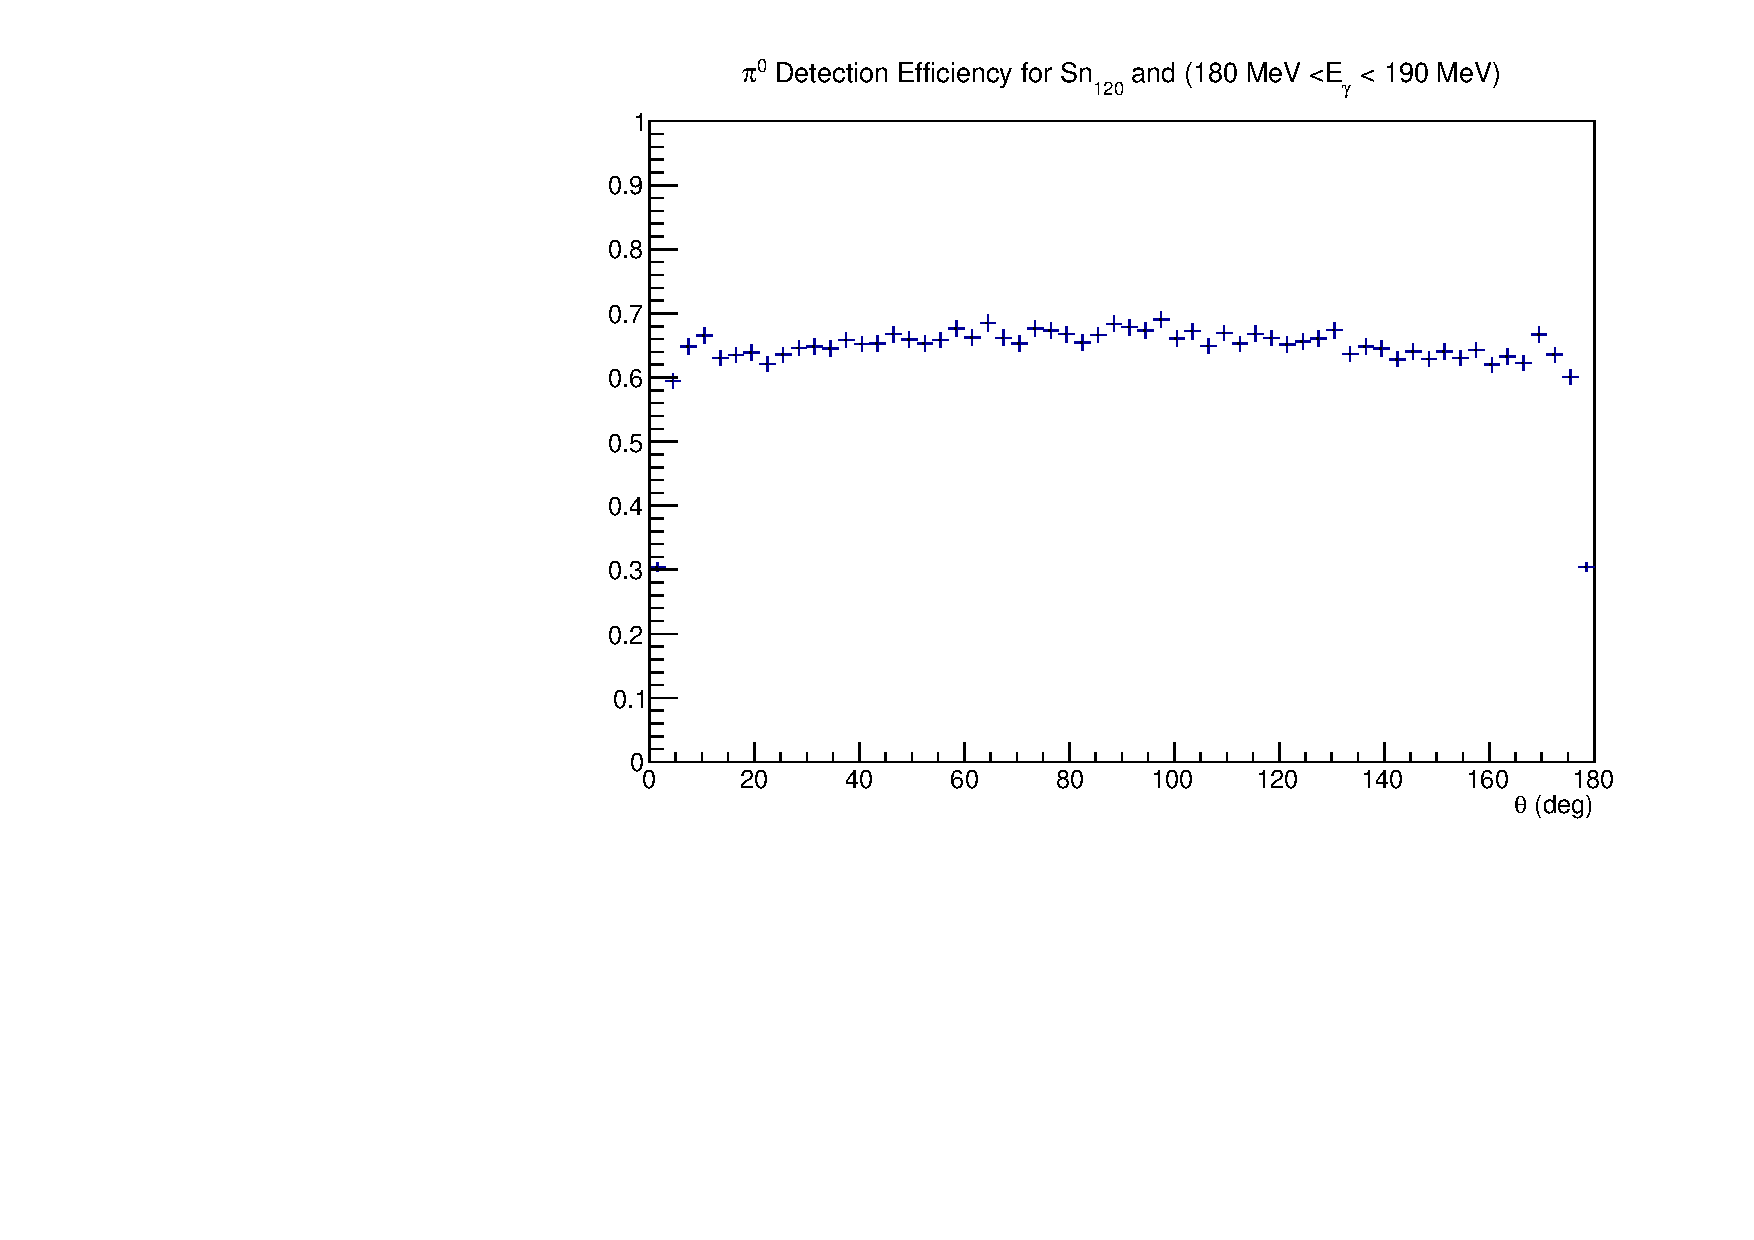
\includegraphics[scale=0.4]{pictures/pdf/pi0_efficiency_Sn120_Ebin6.pdf}
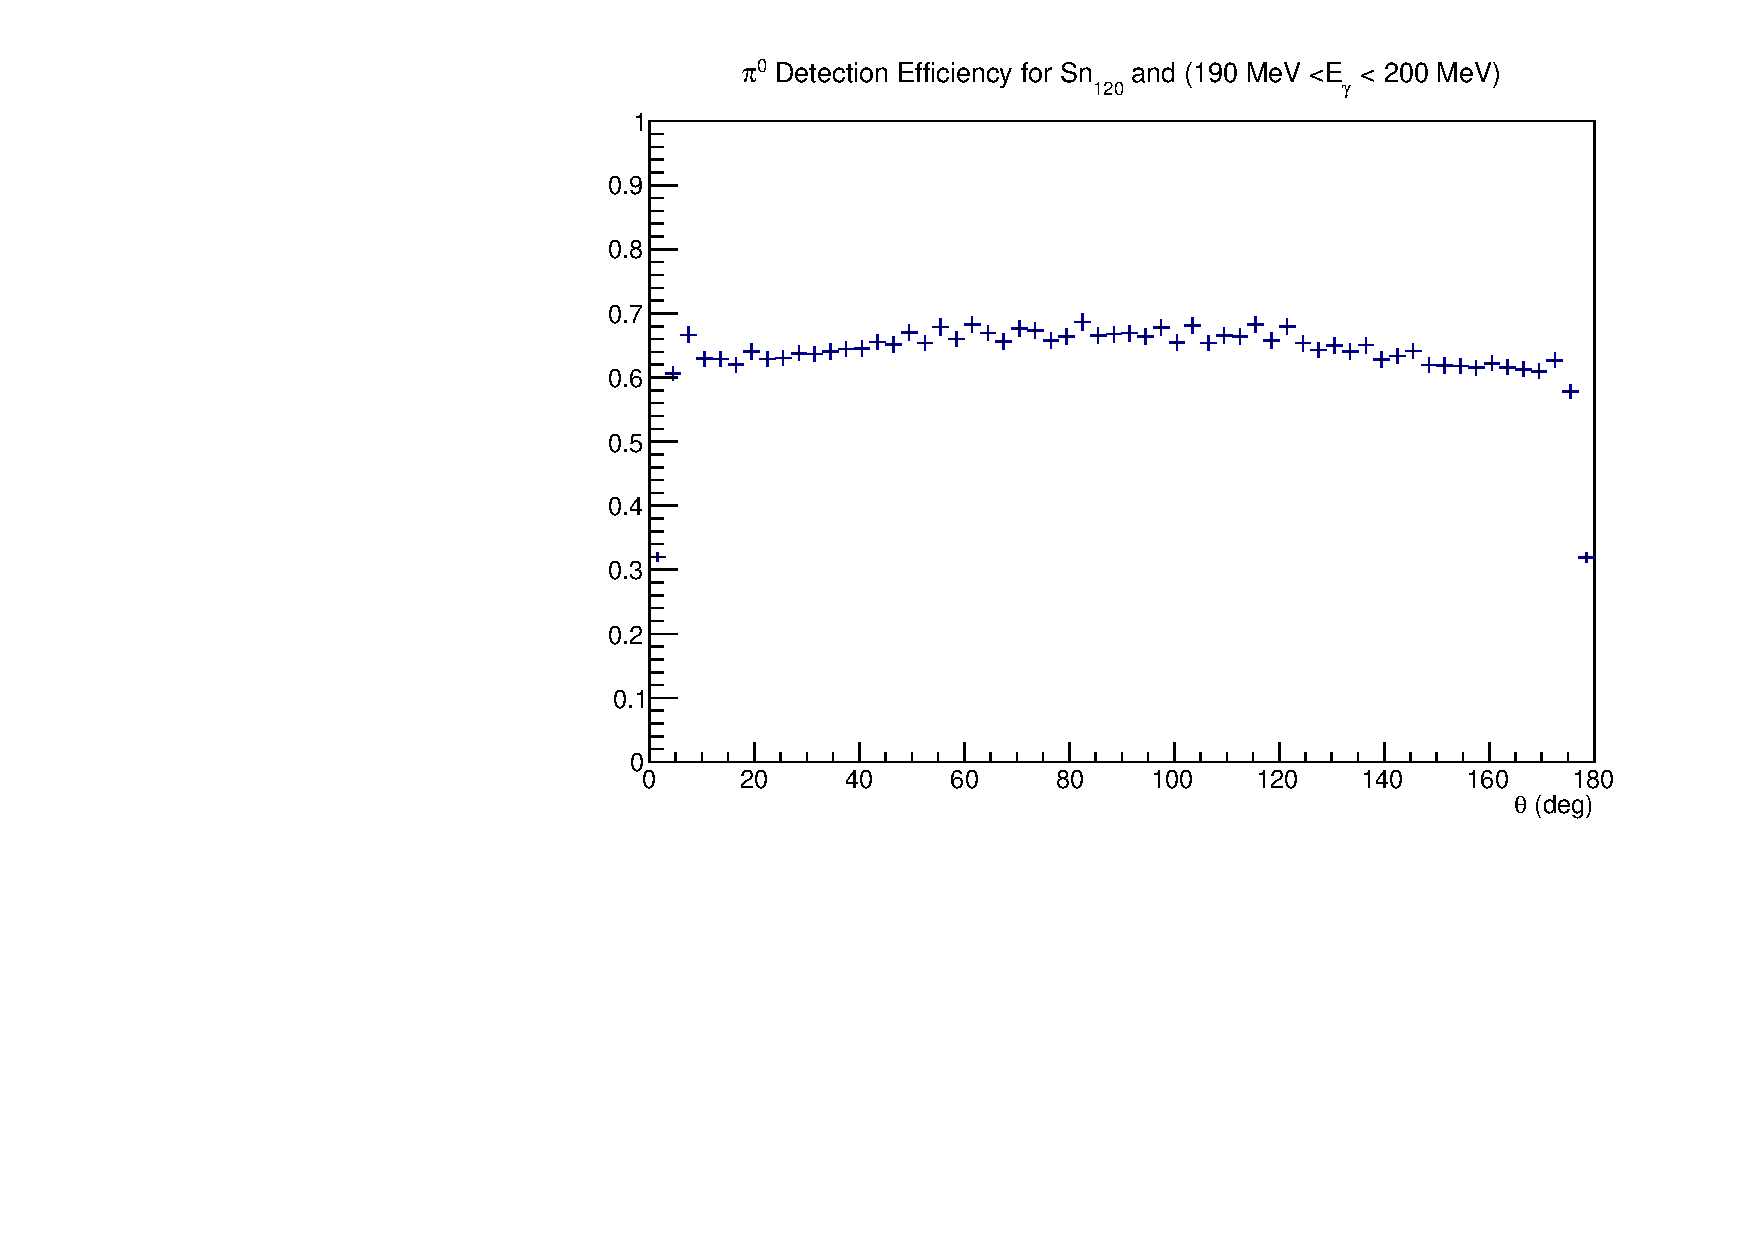
\includegraphics[scale=0.4]{pictures/pdf/pi0_efficiency_Sn120_Ebin7.pdf}
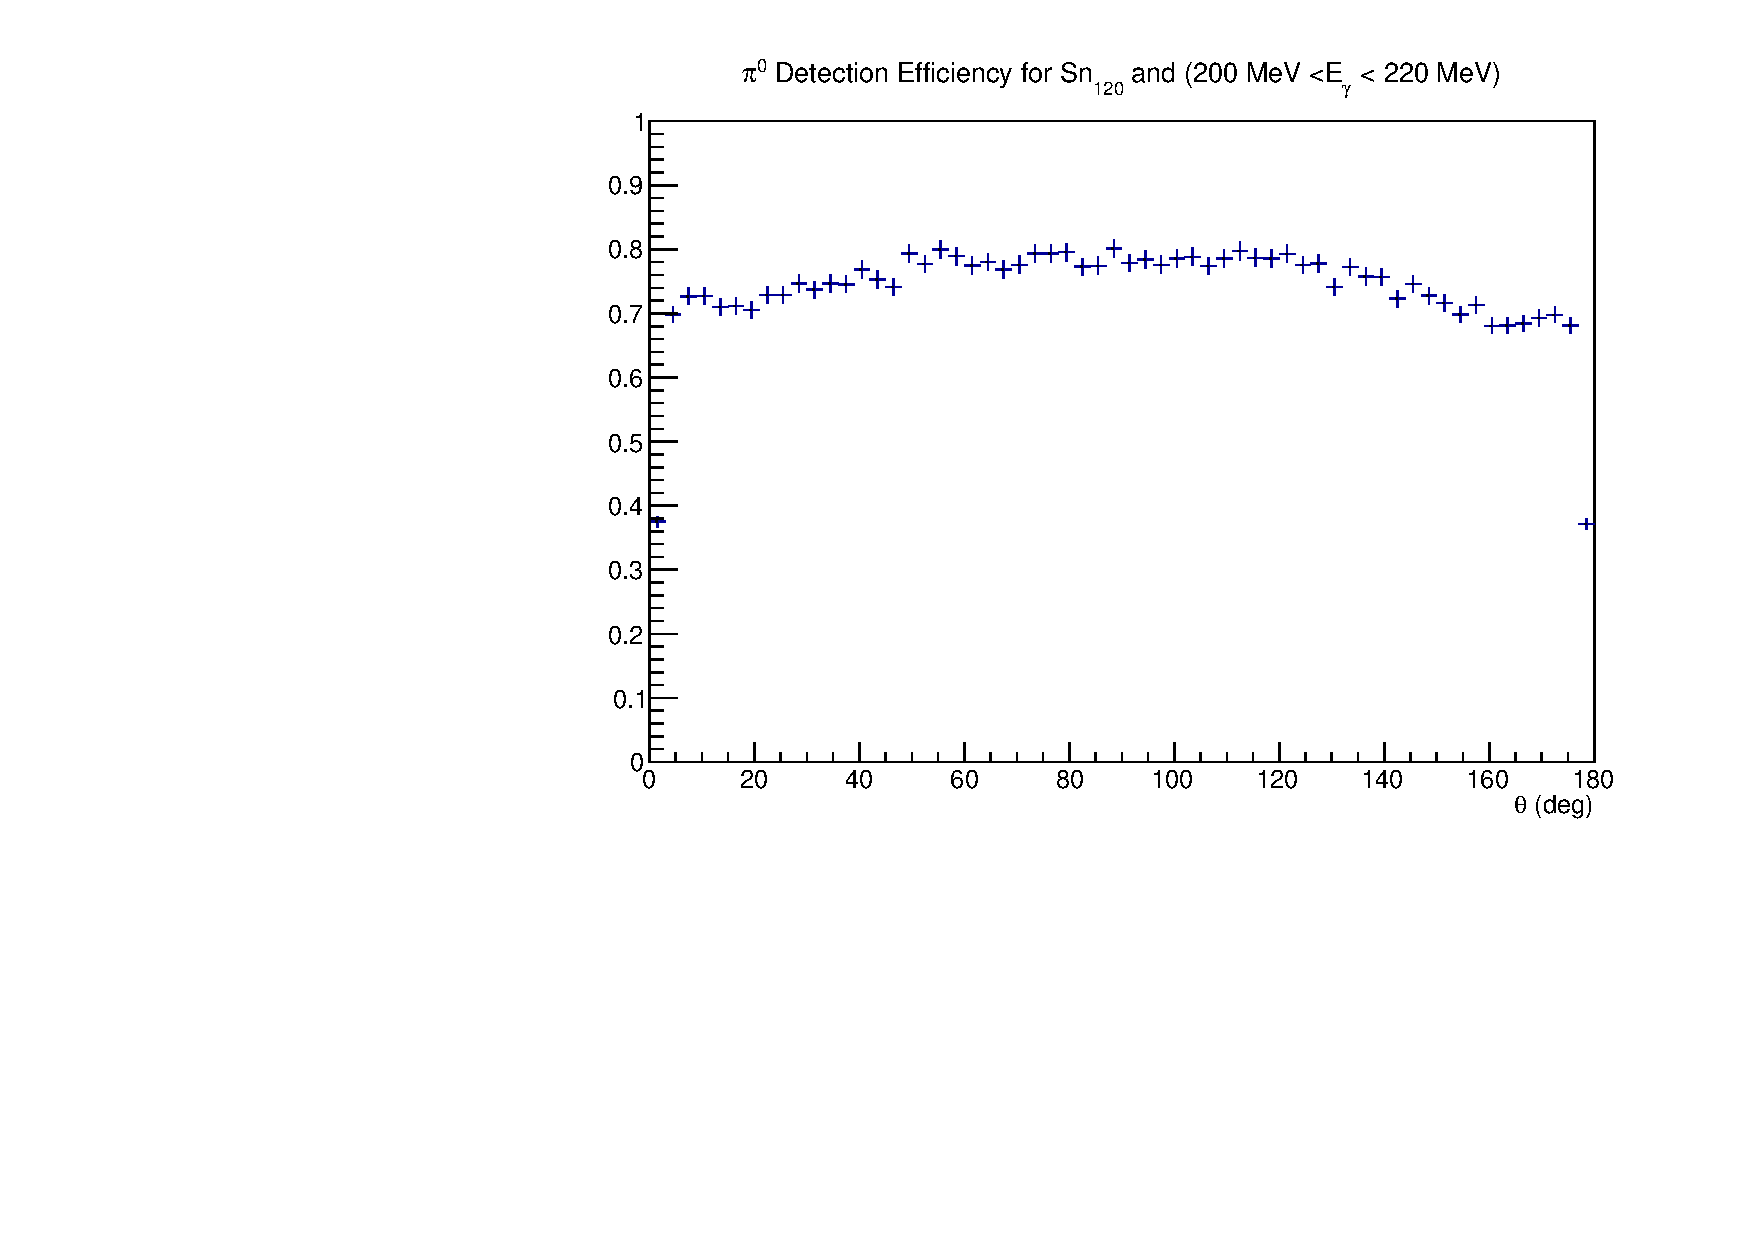
\includegraphics[scale=0.4]{pictures/pdf/pi0_efficiency_Sn120_Ebin8.pdf}
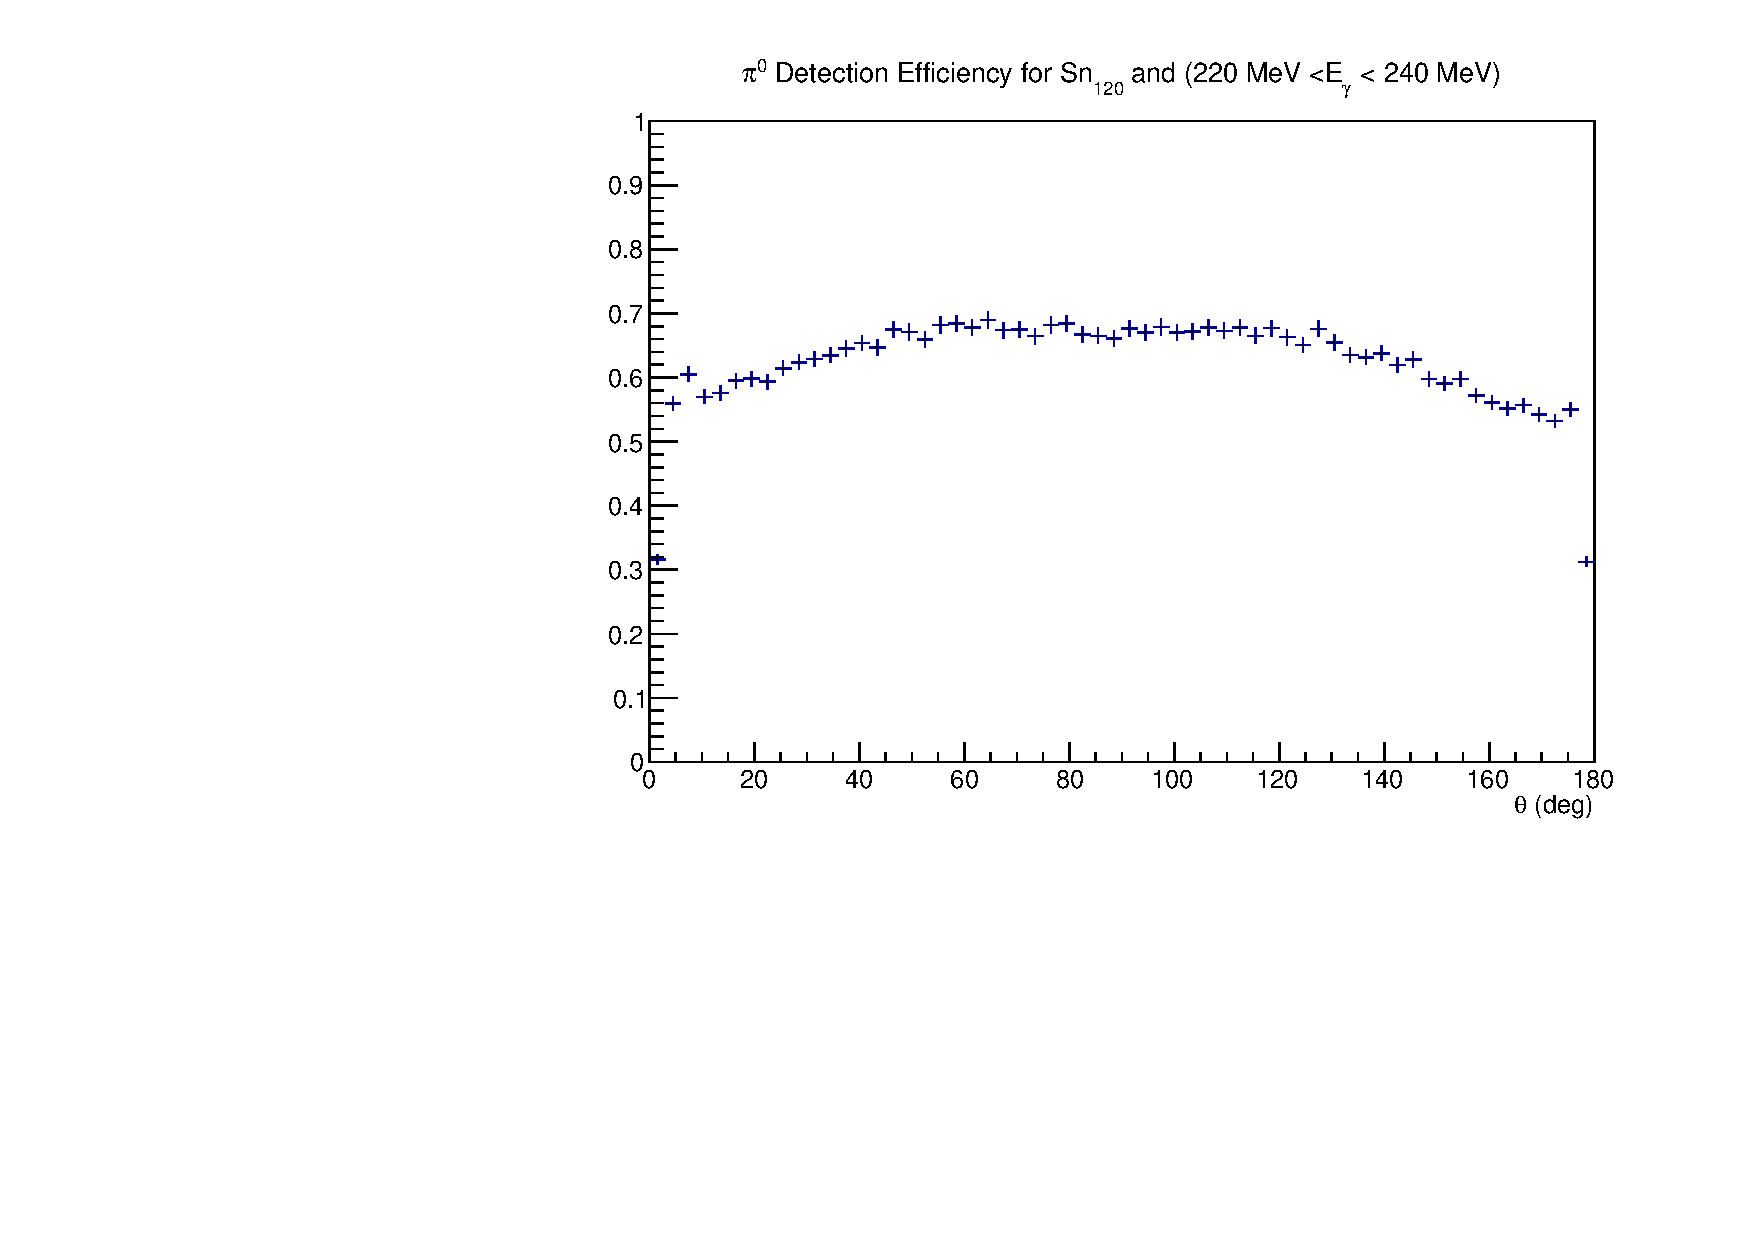
\includegraphics[scale=0.4]{pictures/pdf/pi0_efficiency_Sn120_Ebin9.pdf}
\caption{Dependence of the detection efficiency on energy and $\theta_{\pi^{0}}$ for the $^{120}Sn$ target.}
\label{detectioneff2}
\end{center}
\end{figure}

\begin{figure}[H]
\begin{center}
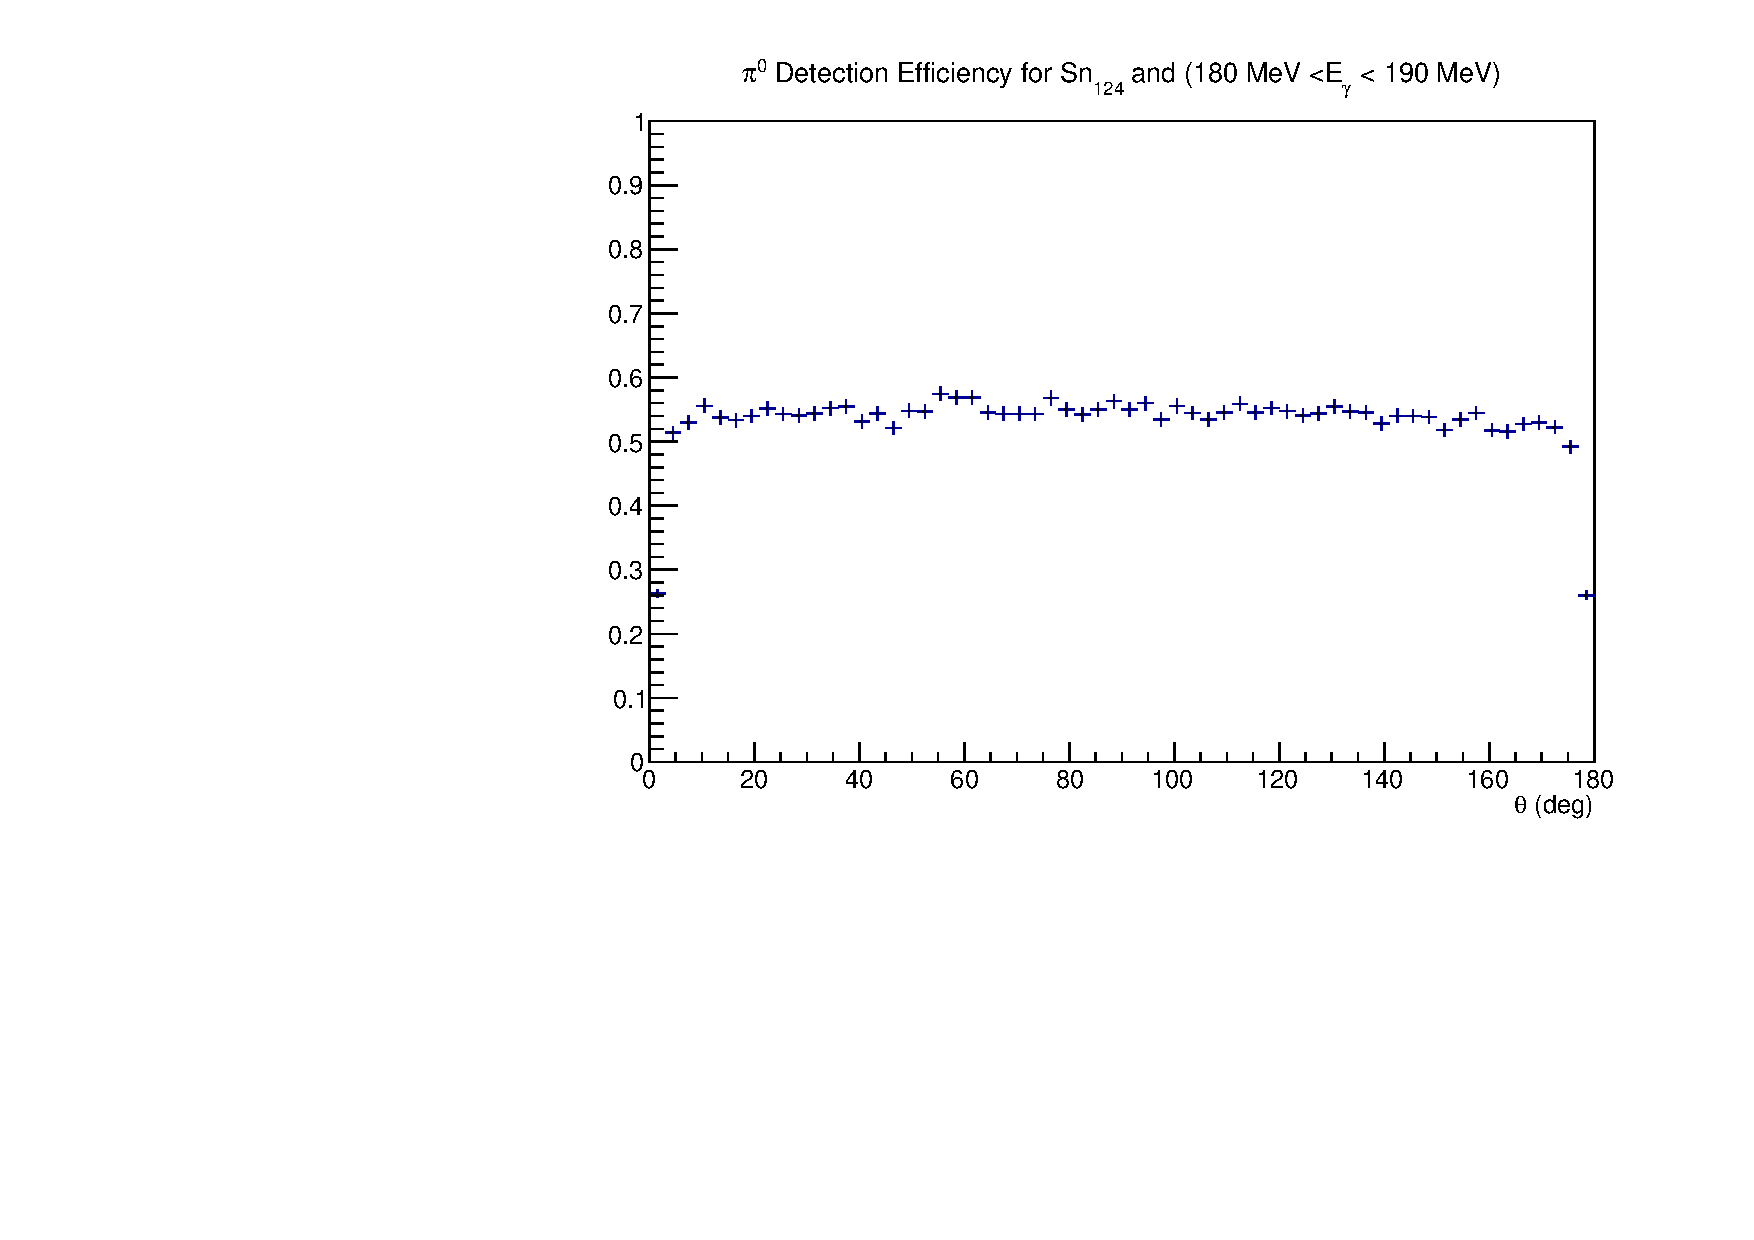
\includegraphics[scale=0.4]{pictures/pdf/pi0_efficiency_Sn124_Ebin6.pdf}
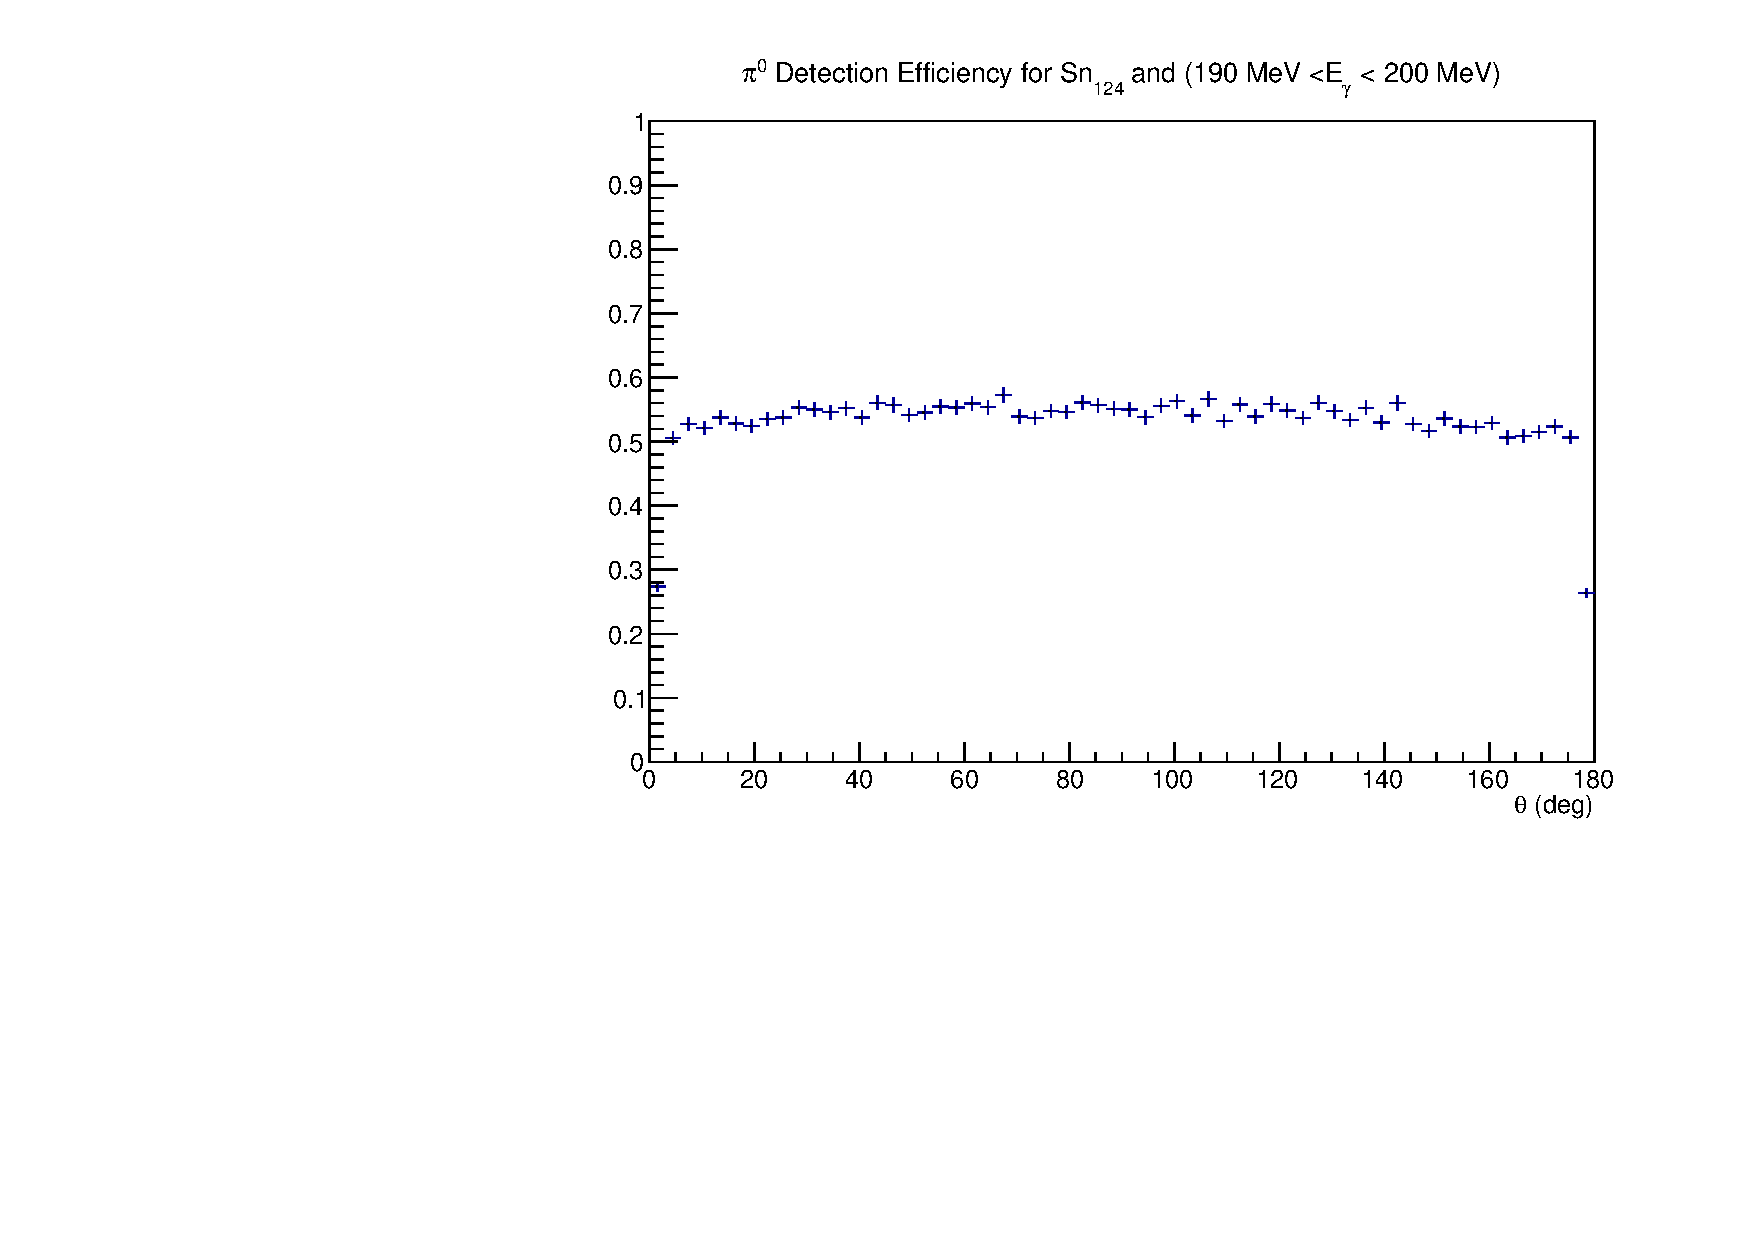
\includegraphics[scale=0.4]{pictures/pdf/pi0_efficiency_Sn124_Ebin7.pdf}
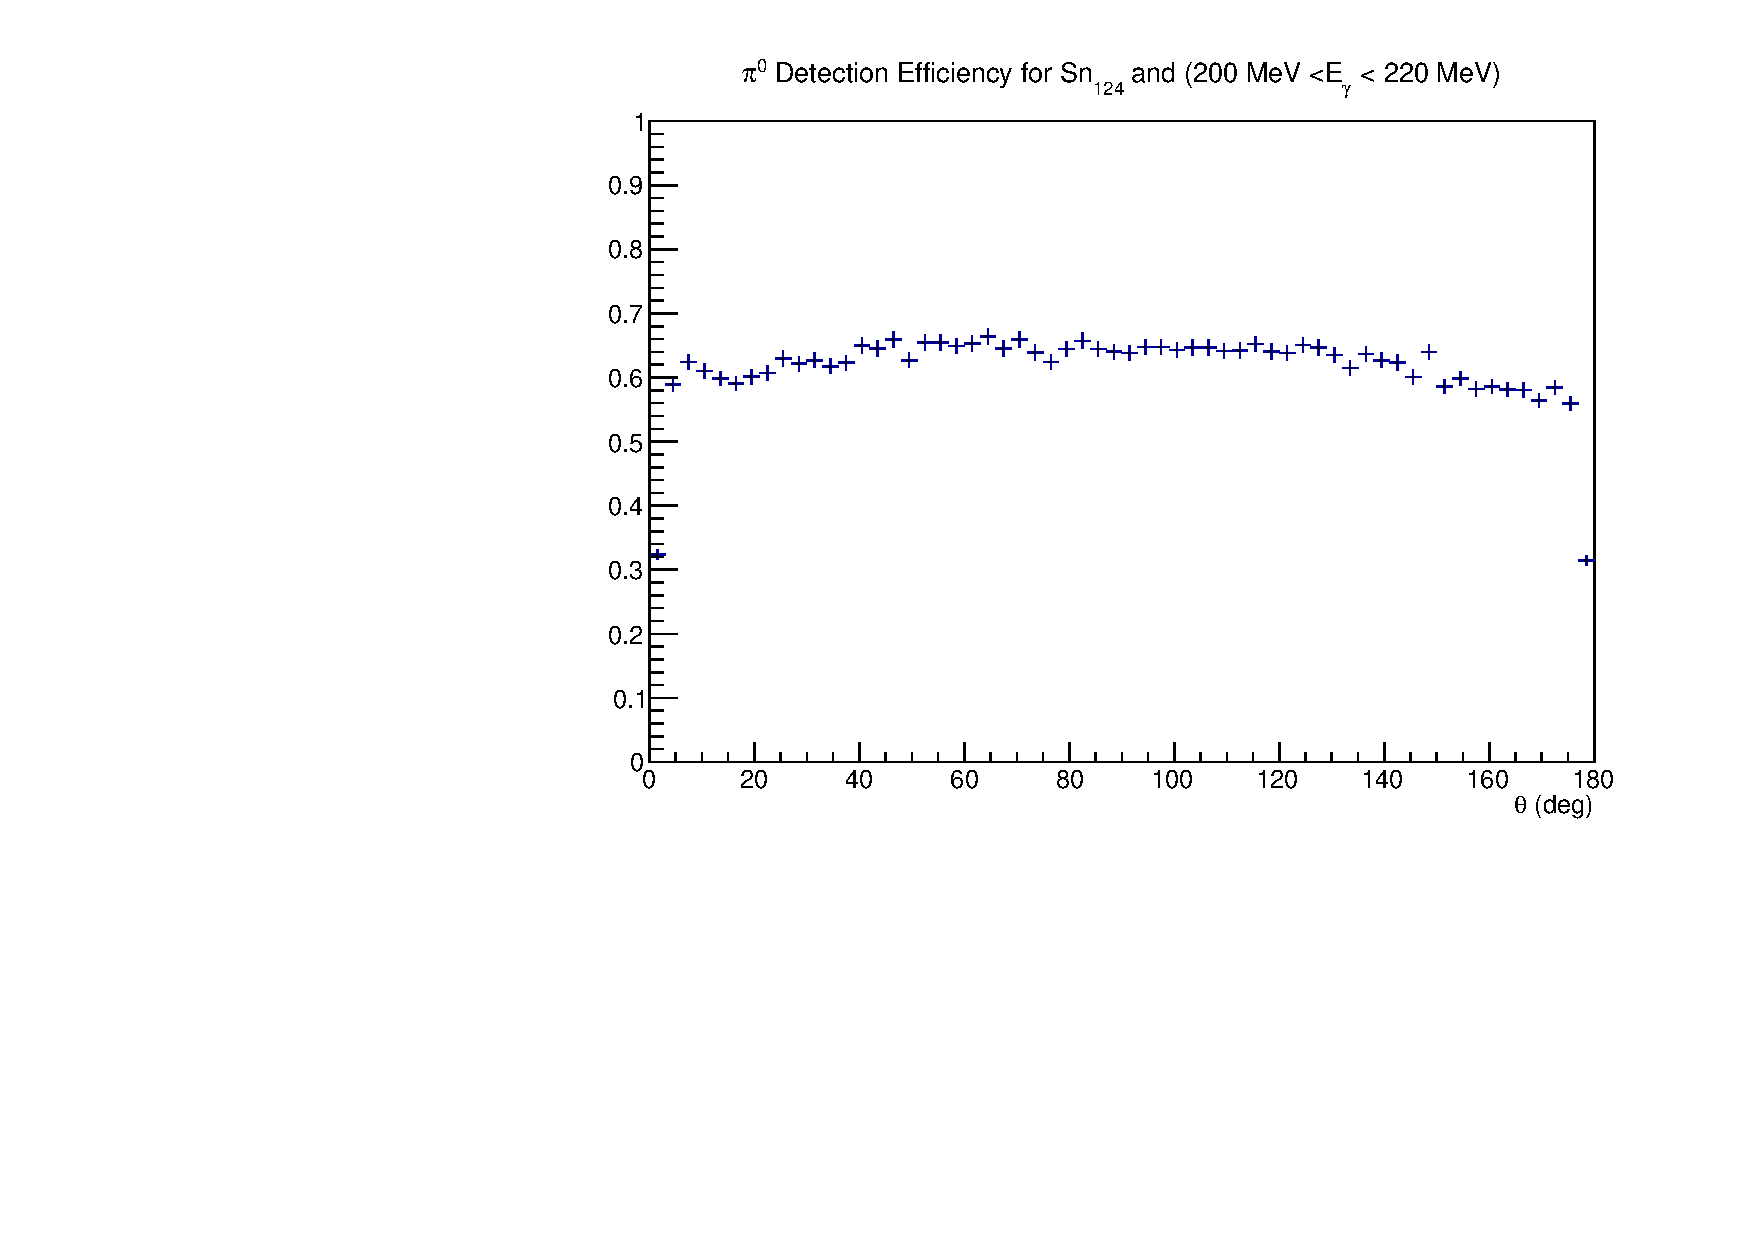
\includegraphics[scale=0.4]{pictures/pdf/pi0_efficiency_Sn124_Ebin8.pdf}
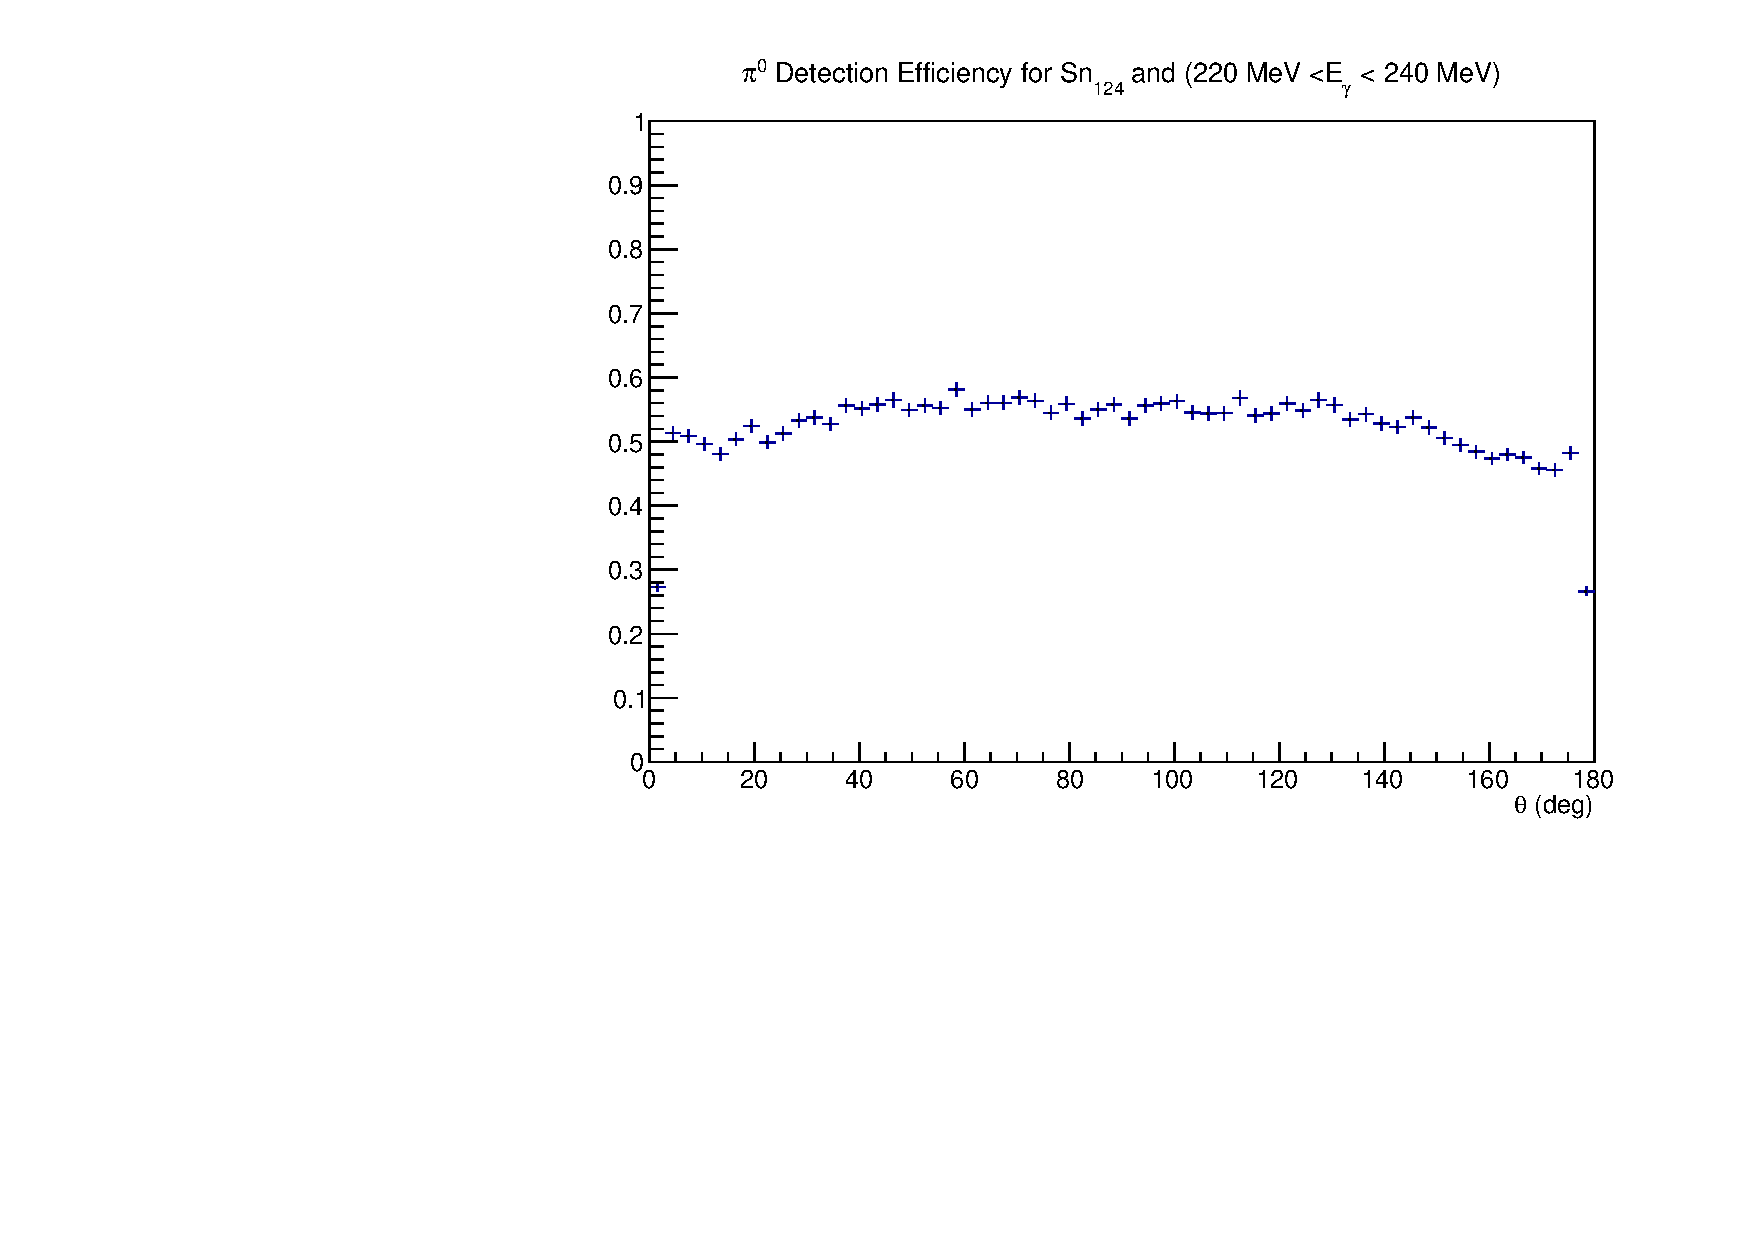
\includegraphics[scale=0.4]{pictures/pdf/pi0_efficiency_Sn124_Ebin9.pdf}
\caption{Dependence of the detection efficiency on energy and $\theta_{\pi^{0}}$ for the $^{124}Sn$ target.}
\label{detectioneff3}
\end{center}
\end{figure}



%\indent The Kamalov's calculations using the predictions of the relativistic mean field FSU-Gold models have been carried out and the predictions of the models have been compared with the experimental results. Before the models could have been compared with the data, calculations had to be smeared with the energy resolution. The dependence of the energy resolution on $\theta$ is shown in the below figure:

%\begin{figure}[H]
%\begin{center}
%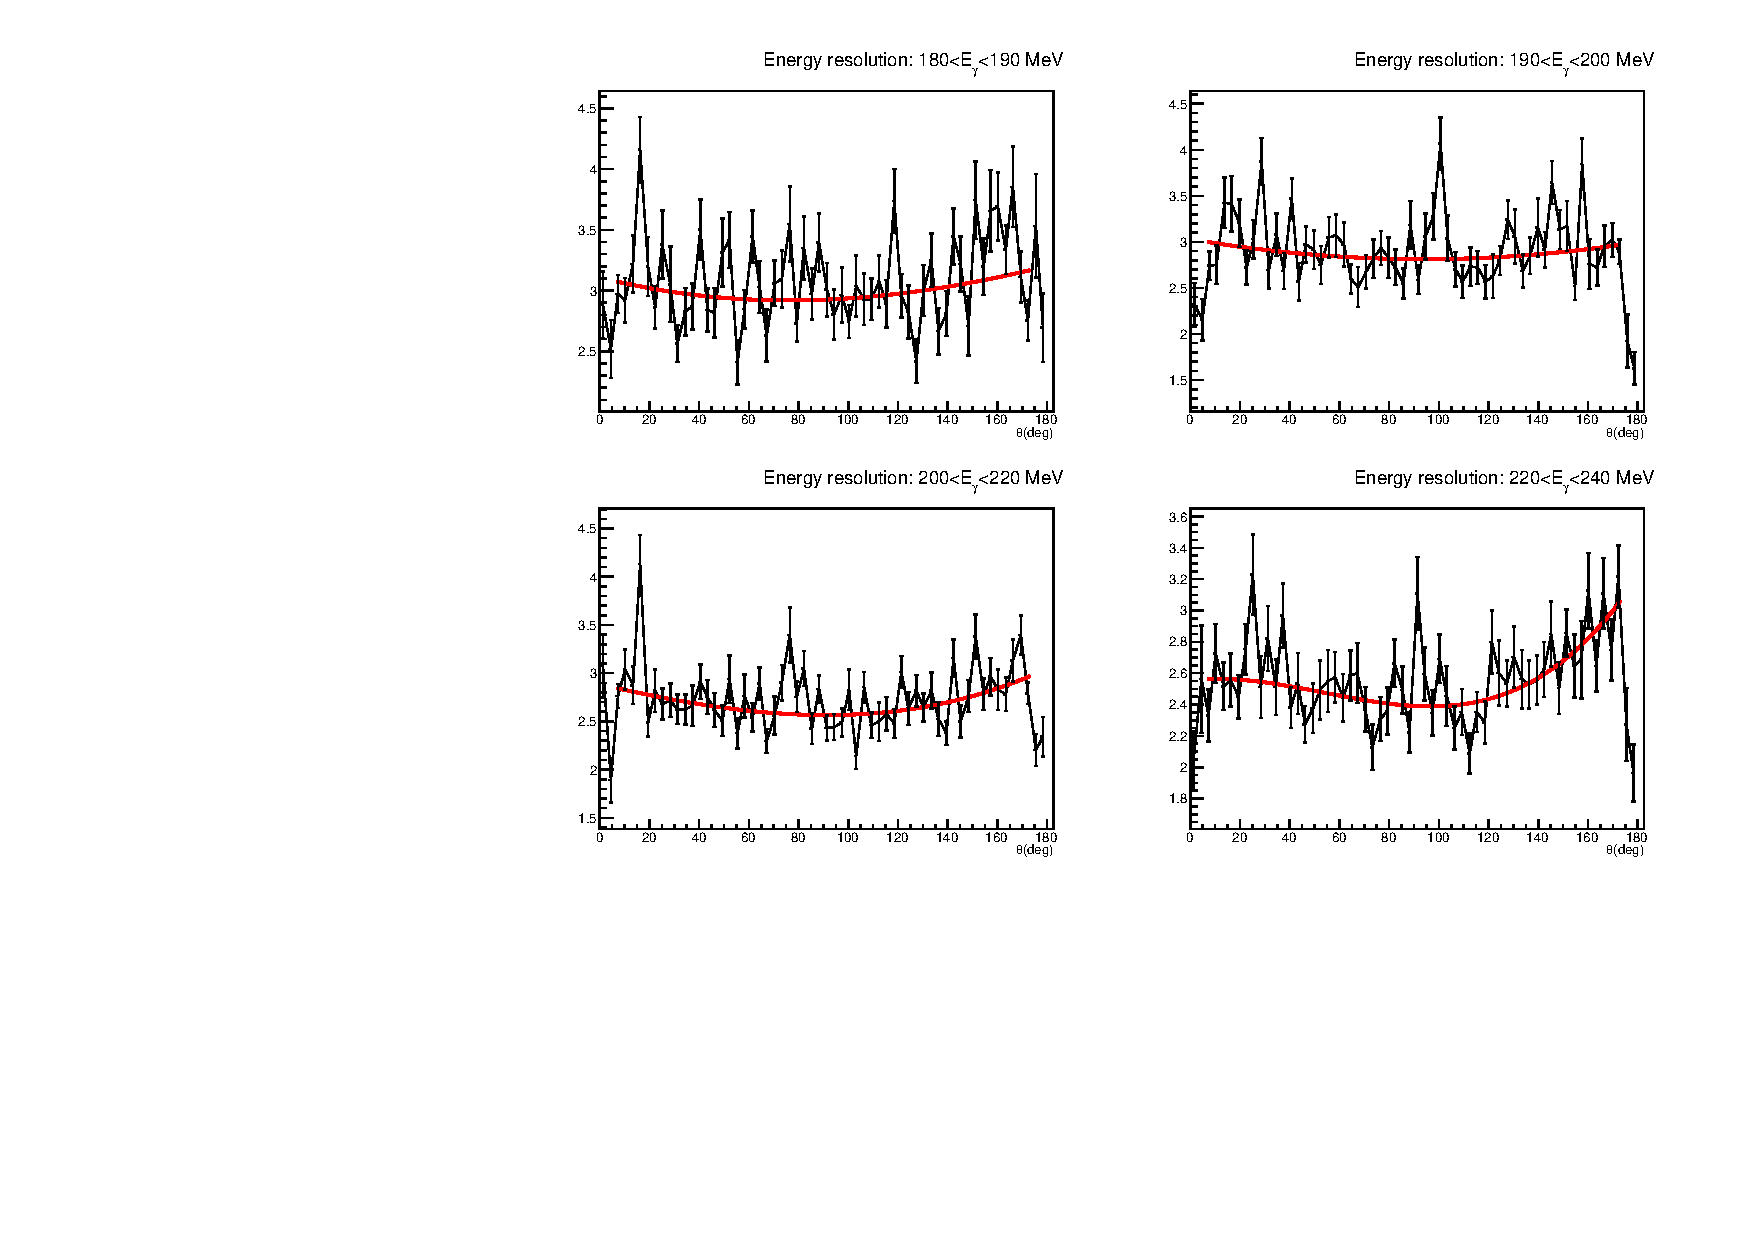
\includegraphics[scale=0.75]{pictures/pdf/energy_resolution_sn116.pdf}
%\caption{Plots of the energy resolution for different energy bins for $^{116}Sn$. Red line is the polynomial fit.}
%\label{energy_res1}
%\end{center}
%\end{figure}

%\begin{figure}[H]
%\begin{center}
%\includegraphics[scale=0.8]{pictures/pdf/energy_resolution_sn120.pdf}
%\caption{Plots of the energy resolution for different energy bins for $^{120}Sn$. Red line is the polynomial fit.}
%\label{energy_res2}
%\end{center}
%\end{figure}

%\begin{figure}[H]
%\begin{center}
%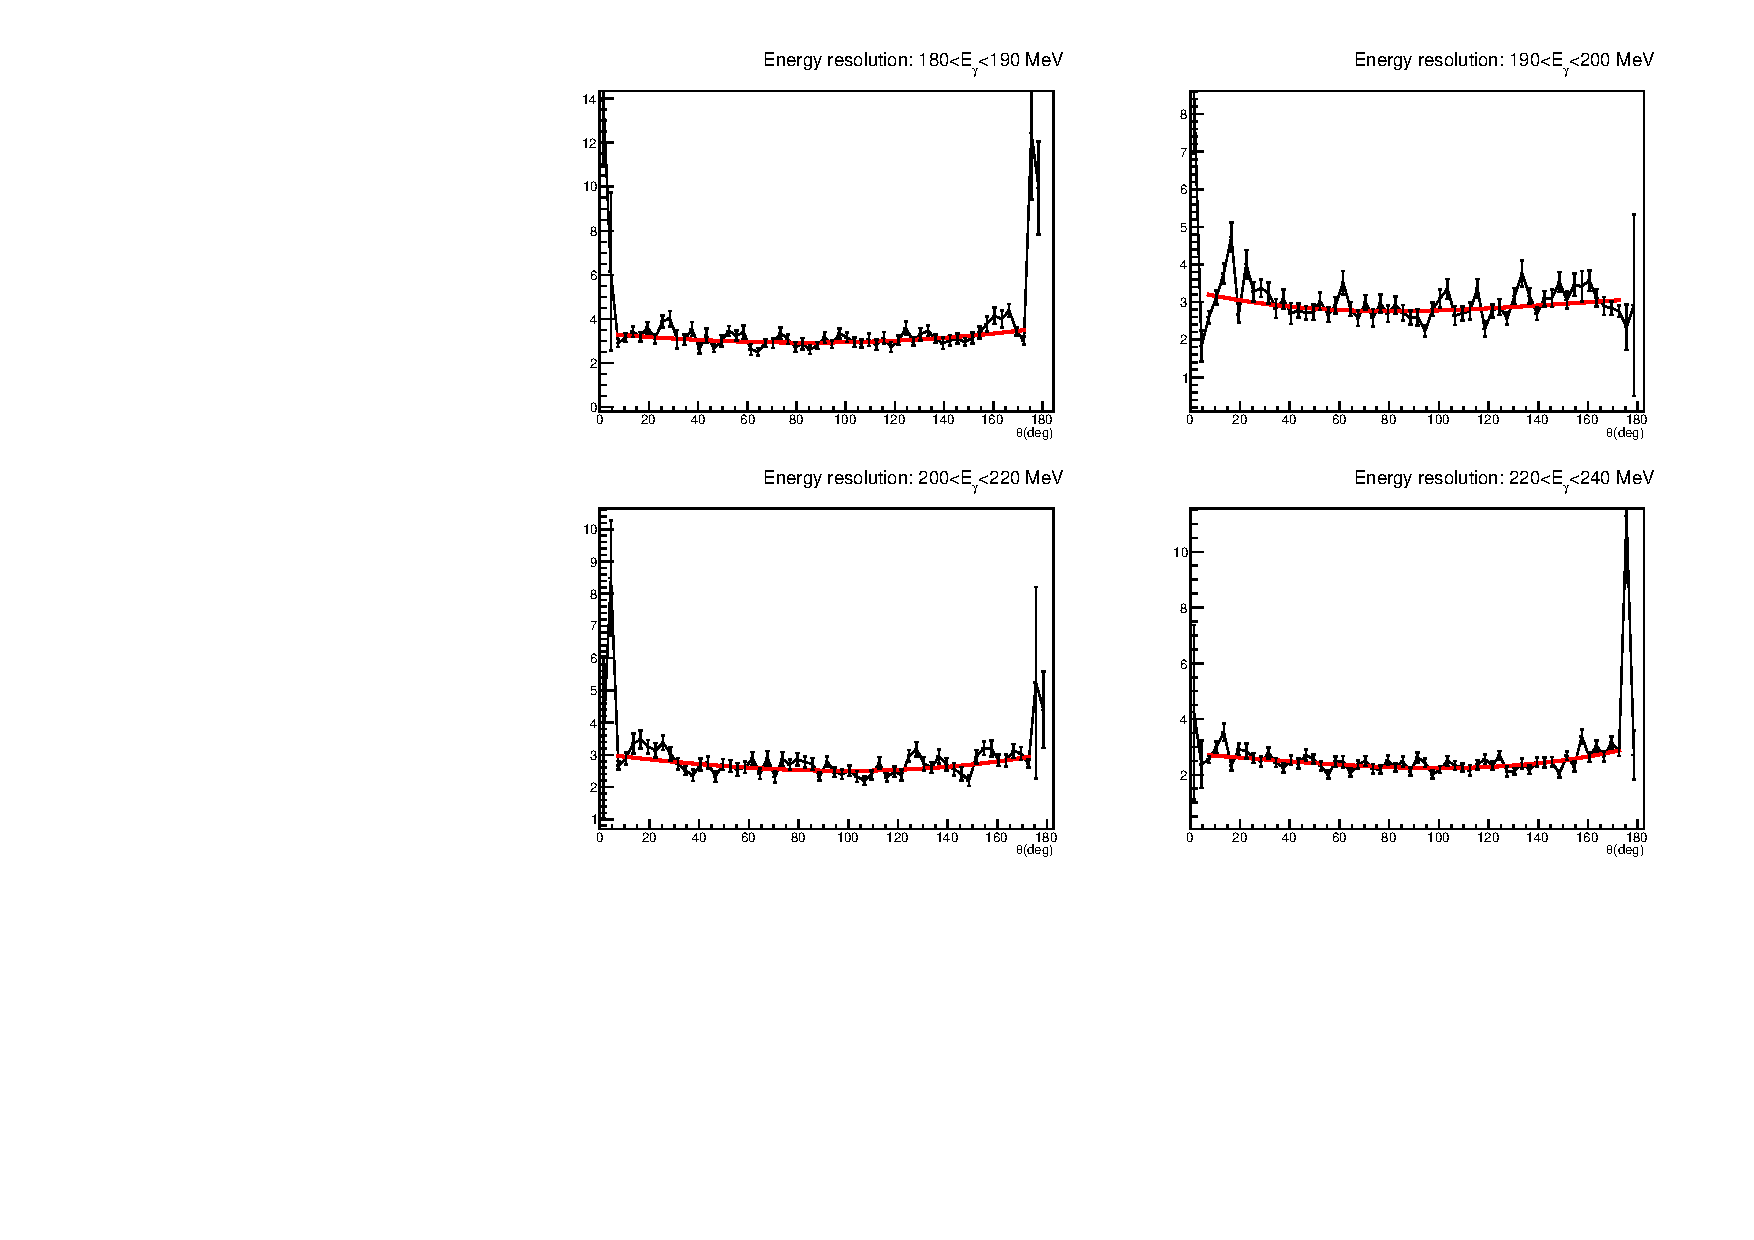
\includegraphics[scale=0.75]{pictures/pdf/energy_resolution_sn124.pdf}
%\caption{Plots of the energy resolution for different energy bins for $^{124}Sn$. Red line is the polynomial fit.}
%\label{energy_res3}
%\end{center}
%\end{figure}

%\indent The energy resolution plots have been fitted with a polynomial function and the value of the energy resolution have been calculated for each $\theta$, for each energy bin. Next, the results of the Kamalov's calculations have been smeared with the energy resolution obtained from the fits and compared with the experimental results (Fig. \ref{smearedratio}).

%\begin{figure}[H]
%\begin{center}
%\includegraphics[scale=0.55]{pictures/pdf/.pdf}
%\caption{Plots of the ratio of yields. Red line is Kamalov's calculations.}
%\label{smearedratio}
%\end{center}
%\end{figure}

\section{Cross Sections Measurements}

\indent The measurement of the cross section is an important way to compare and contrast various theories with the experimental results. From the definition, cross section is a measure of probability that a certain reaction will take place under specified conditions. For a reaction $A(a,b)B$ is defined as:

\begin{equation}
\sigma = \frac{N_{b}}{N_{a}N_{A}}
\end{equation}
where, $N_{a}$ is the number of inicident particles per unit are, $N_{A}$ is the number of target particles per unit area visible to the beam and $N_{b}$ is the number of emitted partices.

\indent In this experiment, $N_{a}$ is the incident photon flux calculated from the number of hits in the tagger scalers corrected with the tagging efficiency, $N_{A}$ is the surface density of the target as seen by the beam, and $N_{b}$ is the $\pi^{0}$ yield corrected with the detection efficiency.

\indent The differential cross section is a derivative of the total cross section with respect to the solid angle. For a given photon energy bin, $E_{\gamma}$, and pion scattering angle, $\theta_{\pi^{0}}$, it can be expressed as:

\begin{equation}
\frac{d\sigma}{d\Omega} = \frac{N_{\pi^{0}}}{N_{s}\epsilon_{tagg}\epsilon_{det}\rho_{a}\Omega\Gamma_{\gamma\gamma}}
\end{equation}
where, $N_{\pi^{0}}$ is the number of $\pi^{0}$'s detected in the given $E_{\gamma}$ and $\theta_{\pi^{0}}$ bins. $N_{s}$ is the number of scalers in the given $E_{\gamma}$ bin. $\epsilon_{tagg}$ is the tagging efficiency in the given $E_{\gamma}$ bin and $\epsilon_{det}$ is the detection efficiency in the given $E_{\gamma}$ and $\theta_{\pi^{0}}$ bins. $\rho_{a}$ is the target surface density in $nuclei/cm^{2}$. $\Gamma_{\gamma\gamma}$ is the branching ratio of the decay, and $\Omega$ is the solid angle of detection, defined as:

\begin{equation}
\Omega = \int_{\phi_{1}}^{\phi_{2}} d\phi \int_{\theta_{1}}^{\theta_{2}}sin\theta d\theta
\end{equation}

\section{Error Analysis}

\indent The cross section calculations are laden with the systematical and statistical uncertainties.

\indent Systematic errors are uncertainties in the bias of the data \cite{leo}. A simplest example would be an offset of the measuring instrument, contrary to the random errors where each measurement fluctuates independently of the others, in case of systematical uncertainty, the entire data set is affected in exactly the same way.

\indent In this experiment, one of the sources of the systematic error is the uncertainty due to the surface density calculations. It arises from the target thickness measurements, and for the $^{116}Sn$ and $^{124}Sn$ targets, it is of order $\sim 1\%$ and for the $^{120}Sn$ target it is $\sim 2\%$.

\indent Another source of systematic error is from the fitting procedure for the $\pi^{0}$ missing energy spectrum. 

\indent There were three sources of the statistical error: the error on the tagging efficiency measurement, the error on the number of $\pi^{0}$'s in each $E_{\gamma}$ and $\theta_{\pi}$ bins and the error on the number of the generated events for the $\pi^{0}$ detection efficiency calculations.

\indent In general, statistical errors arise from the stochastic fluctuations, and in nuclear and particle physics they come from the observation of the Poisson distributed data. In such case, the error decreases with the increasing number of measurements.

\indent The error on the the number of $\pi^{0}$'s in each $E_{\gamma}$ and $\theta_{\pi}$ bins have been obtained from the analysis of the $\pi^{0}$ missing energy spectra, where in the coherent peak the error was of order $\sim 1\%$. The statistical error here comes from the number of the detected $\pi^{0}$'s and statistical uncertainty associated with the tagger random subtraction.

\indent The uncertainty in the number of the generated events for the detection efficiency calculations have been chosen so the error on detection efficiency is no greater than the error on the number of $\pi^{0}$'s in each $E_{\gamma}$ and $\theta_{\pi}$ bins, i.e. $\sim 1\%$.

\indent The systematic error on the tagging efficiency measurement is of order of $\sim 1\%$ for all the channels and all the targets.